\documentclass[10pt,twocolumn]{article}

\usepackage[a4paper,margin=18mm,columnsep=6mm]{geometry}
\usepackage[T1]{fontenc}
\usepackage[utf8]{inputenc}
\usepackage{lmodern}
\usepackage{microtype}
\usepackage{amsmath,amssymb}
\usepackage{booktabs}
\usepackage{array}
\usepackage{graphicx}
\usepackage{xcolor}
\usepackage{url}
\usepackage[hidelinks]{hyperref}
\usepackage{cite}

\graphicspath{{../reports/figures/}{../reports/early_warning/figures/}{../reports/virtual_metrology/figures/}}
\setlength{\parindent}{1em}
\setlength{\parskip}{0pt}
\setlength{\emergencystretch}{2em}

\newcommand{\mrr}{\mathrm{MRR}}
\newcommand{\pending}{\textcolor{orange!70!black}{\textbf{PENDING}}}
\newcommand{\simonly}{\textcolor{blue!55!black}{\textbf{Synthetic-simulation evidence}}}
\newcommand{\native}{\text{native PHM target unit}}

\title{A Simulation-First Framework for Predictive Supervisory Control of CMP under Electrical and Ultrapure-Water Disturbances:\\
Public Virtual Metrology, Physics, Coupling, and Synthetic Early Warning}

\author{Living manuscript for the Semiconductor CMP Predictive-Control PoC\\
\small Journal-neutral draft; author list and affiliations pending}

\date{Evidence freeze: 13 July 2026\\Last manuscript build: \today}

\begin{document}

\maketitle
\begin{center}
\fbox{\parbox{0.91\columnwidth}{\small
\textbf{Evidence boundary.} This living paper reports verified data provenance,
leakage-safe PHM average-MRR virtual metrology, synthetic plant/CMP/coupling
evidence, and the frozen WP12 simulation-only early-warning experiment. The
PHM target unit is source-undeclared and the selected tree's primary intervals
undercover. WP12 has only three independent held-out events and fails under
important structural and observation shifts. Root-cause attribution,
controller efficacy, and safety-filter outcomes remain unavailable. No
real-fab, physical-defect, yield, equipment-protection, or production-control
conclusion is made.}}
\end{center}
\vspace{0.7em}

\begin{abstract}
Chemical mechanical planarization (CMP) depends on process settings,
consumable condition, and utility support. This work develops a
simulation-first proof of concept for studying whether an eventual predictive
supervisory layer can warn of and mitigate simulated material-removal-rate
(MRR) excursions caused by electrical and ultrapure-water (UPW)
disturbances. The intended chain is electrical disturbance, UPS and
variable-frequency-drive response, motor and pump response, UPW hydraulic and
thermal response, an explicitly declared CMP boundary, and finally a change
in simulated MRR. The PHM 2016 CMP archive was locally supplied,
integrity-checked, selectively extracted, and audited. A leakage-safe offline
comparison uses 311/275 precedence-retained test/final-validation records from
mutually disjoint wafers in the source-native target scale. A tree selected
before holdout access attains MAE 3.185/3.395 and $R^2$ 0.975/0.958, reducing
MAE by 89.2\%/88.6\% relative to a mean baseline. Its nominal 90\%
split-conformal intervals cover only 83.9\%/84.7\%, below a frozen 85\%
interpretation floor, and a chronological stress is dominated by one
preregistered extreme label. The physics-plus-residual hybrid is significantly
worse than the tree, so no hybrid-improvement claim is supported. A
reduced-order CMP subsystem
implements explicit process modes, signed rotary kinematics, generalized
pressure--velocity exposure, dynamic consumable and slurry states, an
interface energy balance, and cumulative removal. Its nominal reference is
100 nm/min at 30 kPa and passes limiting-case, dimensional, energy-residual,
quadrature, replay, and timestep-refinement checks. A typed stateless coupler
implements no connection, dressing-water support, a conditional thermal loop,
and an explicitly synthetic slurry-support structure. A healthy-UPS 25\%,
400 ms voltage sag is an exact coupling negative control. In a separately
declared synthetic stress test, a 500 J degraded-UPS interruption during
dressing drives pump and UPW support to zero, reduces end-of-dress pad activity
by 5.36\%, and reduces mean MRR during later polishing by 3.19\% relative to an
otherwise identical no-connection run. This delayed effect is mediated by pad
state, not a direct UPW-to-MRR multiplier. Global and mismatch analyses show
material dependence on synthetic topology and coefficients. These results
establish a testable synthetic plant and coupling basis. A separately frozen
warning target predicts whether active-POLISH MRR will leave a paired-reference
$\pm5\%$ band persistently for 0.25 s within a 3 s horizon. Across 24 held-out
synthetic runs containing only three independent events, logistic regression
achieves PR-AUC 0.9904 and the gradient-boosted model 0.9130; both detect 3/3
events with 2.71 s median lead. However, both alarm severely when upstream
events are replayed under no CMP connection, and high synthetic noise degrades
discrimination and uncertainty coverage. The warning result is therefore
limited to the named primary ensemble and does not establish predictive-control
efficacy, real-tool calibration, or topology-independent applicability.
\end{abstract}

\noindent\textbf{Keywords:} chemical mechanical planarization; material
removal rate; ultrapure water; reduced-order modelling; virtual metrology;
early warning; supervisory control; sensitivity analysis; simulation

\section{Introduction}

CMP combines mechanical contact, relative motion, slurry chemistry, pad
condition, and heat transfer to remove material. Pressure--velocity
proportionality provides a classical starting point
\cite{preston1927}, but process dynamics and conditioning history make an
instantaneous algebraic model insufficient for disturbance and control
studies. Kinematics affect local exposure \cite{hocheng2000}; pad wear and
conditioning introduce state memory \cite{borucki2002,borucki2004,chang2007};
and slurry and temperature can alter the process through distinct pathways
\cite{white2003,mudhivarthi2006,bahr2017}.

The central research question is whether a predictive supervisory-control
layer can detect an upcoming simulated CMP excursion caused by electrical and
UPW disturbances and reduce it relative to no intervention and fixed-threshold
control without violating predefined simulation constraints. Answering that
question requires more than fitting a predictor. The upstream plant must obey
energy and hydraulic balances, the connection into CMP must be explicit, the
true latent state must remain distinct from delayed and corrupted observations,
and controller comparisons must be paired on identical disturbances and seeds.

This manuscript is intentionally staged. The completed contribution comprises
a leakage-safe PHM average-MRR comparison, a scientifically bounded synthetic
plant, a declared utility-to-CMP connection with null controls and sensitivity,
and an open-loop early-warning experiment with disjoint run-level
fitting/calibration roles. Attribution, predictive control, safety filtering,
and the integrated comparison remain protocols until their acceptance evidence
exists.

The present contributions are:
\begin{enumerate}
  \item a data and claims contract that separates measured process output,
  simulated physical state, observed sensor state, process excursion,
  quality-risk proxy, physical defect, and yield outcome;
  \item a target-blind whole-wafer split, six-family source-native virtual-
  metrology comparison, grouped uncertainty analysis, and explicit label,
  feature-proxy, continuity, and chronological sensitivities;
  \item a reduced-order utility and CMP simulator with conserved UPS energy,
  hydraulic mass balance, explicit process modes, cumulative removal, and
  causal observation clocks;
  \item a typed topology map that replaces an earlier direct UPW-to-MRR gain
  with bounded dressing-water, thermal, synthetic slurry-support, and null
  structures; and
  \item negative-control, positive-chain, numerical, structural, local,
  global, and mismatch evidence for the synthetic plant and coupling;
  \item a frozen active-POLISH early-warning target, causal arrived-signal
  feature boundary, disjoint probability/conformal calibration, held-out
  warning metrics, target sensitivity, and explicit structural/noise failures.
\end{enumerate}

\section{Evidence taxonomy and claim boundary}

The primary measured target is average MRR, denoted
$\widehat{\mrr}$. The simulator may derive excursion probability,
under-polish or over-polish risk, a hold requirement, and spatial proxies.
Without measured spatial metrology, every spatial output is labelled exactly:
\emph{Simulated spatial-uniformity proxy; not experimentally validated
WIWNU}.

Two evidence planes are kept dimensionally separate. The SI simulator uses Pa,
m$^3$/s, m/s, K, s, and m. The PHM model predicts a stage-average target in
the source's native numeric unit because the original source does not declare
the target unit and its process columns use hidden scaling factors. An SI
physics prediction cannot be added to a residual fitted on scaled PHM inputs
without a separately supported calibration bridge.

The supported claims at this evidence freeze are narrow: one selected tree
predicts source-native average MRR on the precedence-retained PHM roles; the
synthetic CMP subsystem satisfies its declared equations and invariants;
configured electrical disturbances can propagate through the tested synthetic
utility topology into CMP state; and two frozen models predict one
preregistered simulator excursion target on the named primary ensemble. The
public result has interval undercoverage and temporal fragility; the warning
claim rests on only three held-out events and does not survive all audited
shifts. The study does not claim prediction or prevention of physical defects, real
wafer-yield loss, real equipment damage, controller benefit, or readiness for
production control. Feature attribution, when later implemented, will not be
described as causal proof.

\section{Scientific basis and topology selection}

The model begins from Preston-type pressure--velocity proportionality
\cite{preston1927} and signed relative-velocity kinematics
\cite{hocheng2000}. Pad asperity wear motivates a stored surface-activity state
\cite{borucki2002}; conditioning and polishing jointly evolve that state
\cite{borucki2004,chang2007}; and conditioner geometry or wear motivates a
separate dresser-effectiveness state \cite{sun2010,kim2017}.

The local literature supports three qualitatively distinct water-related
pathways. First, DI water is used during pad conditioning, and conditioning
temperature can affect later polishing in the studied apparatus
\cite{kim2005,mudhivarthi2006}. This supports a delayed pathway from an
explicit conditioning-water branch to realized dressing, pad state, and later
MRR. Second, rinse water can mix with fresh and spent slurry, so a change in
rinsing has competing dilution, debris-removal, and slurry-availability effects
\cite{bahr2017}; its sign is not safely represented by a universal monotone
gain. Third, lumped heat storage and slurry heat removal are physically
meaningful \cite{white2003}, but the reviewed literature does not establish
that a facility UPW header feeds the target tool's coolant loop.

Accordingly, dressing-water support is the primary connected synthetic
topology. A thermal loop and a specifically named synthetic slurry-support
topology are structural alternatives. No connection is the default and a
mandatory negative control. The reviewed papers do not calibrate
facility-header pressure or flow thresholds, establish the plumbing of the
PHM challenge tool, or justify transferring material-specific numerical
effects into this simulator.

\section{Data provenance and preprocessing contract}

\subsection{Archive evidence}

The PHM 2016 CMP archive \cite{phm2016cmp} was supplied locally rather than
downloaded by the project. The 17,399,074-byte compressed archive has SHA-256
\texttt{976b2310\ldots 12a1eb9}; all members passed ZIP CRC testing. Selective
extraction retained 558 original members: 185 training, 185 test, and 185
validation time-series files plus three MRR tables. Answer files and derived
experiments were excluded. Fifty-eight header-only traces remain explicit
empty traces; they were not silently imputed or replaced. A separate licence
for the embedded dataset was not stated by the source, so redistribution and
licensing conclusions are outside this work.

The loader verifies the extraction manifest, file sizes and hashes, exact
25-column time-series headers, three-column MRR headers, identifier presence,
duplicate keys, trace counts, and label joins. Targets remain separate from
predictors until audited one-to-one joins. Test and validation labels are not
joined into fitting features.

\subsection{Time support, process proxies, and anomalies}

Source row order is preserved and continuity segments break at trace
boundaries, non-positive time increments, and gaps exceeding 10 s. Within a
continuous segment, the duration represented by row $i$ is
\begin{equation}
 w_i=\frac{1}{2}\Delta t_{i-1}^{+}
    +\frac{1}{2}\Delta t_{i+1}^{+},
 \label{eq:time-support}
\end{equation}
where only valid positive adjacent increments contribute. This centered
support prevents duplicated timestamps, reversals, or long gaps from receiving
fictitious duration. Five process-mode proxies are derived from inputs only;
they are not represented as measured phase labels.

The processed bundle contains 1,981 training, 424 test, and 424 validation
wafer/stage records, each with 405 target-free predictor columns. All official
joins have zero missing and zero orphan keys. Complete-trace features are
explicitly offline-only. The audit retains three negative time increments in
training, two in validation, 2,907 zero increments, and 2,855 long gaps. It
also records 221, 43, and 42 unresolved wafer/stage groups in training, test,
and validation, respectively.

Before virtual-metrology fitting, a feature-only identity audit found that the
source partitions share 113 training/test, 115 training/validation, and 34
test/validation wafer IDs, always in the opposite stage. We therefore apply
fixed source precedence (training, then test, then validation), retaining
1,981, 311, and 275 rows from 1,699, 302, and 267 mutually disjoint wafers.
The complete 424-row source holdouts remain collision-contaminated descriptive
diagnostics and cannot support independent-wafer generalization claims.

Four training targets lie between 4,129.494 and 4,326.154 while all other
training targets are at most approximately 163. Dividing those four values by
60 would place them between 68.825 and 72.103, but no authoritative source
supports doing so as a factual correction. The preregistered policy is
therefore to retain original labels for the primary analysis, report a
sensitivity excluding the four records, and report a separately labelled
hypothetical divide-by-60 sensitivity. Selection among these treatments based
on holdout performance is forbidden.

Official training is restricted to fitting and tuning; precedence-retained
test is an offline holdout; and precedence-retained validation is the final
public holdout. Inner resampling retains whole wafers and chronological
blocks. A physical-machine holdout is
infeasible because all records use machine ID 2; a varying field named
\texttt{MACHINE\_DATA} is not treated as a stable machine identifier.

\subsection{Public-data result status}

WP09 is complete for offline average MRR in the source-native target scale.
The selected tree beats the mean baseline on both precedence-retained
holdouts, but its primary split-conformal intervals fall below the frozen
coverage floor. The result does not establish physical units, machine
generalization, electrical/UPW causality, streaming performance, or control
utility.

\section{System architecture and causal timing}

Figure~\ref{fig:architecture} shows the completed plant and CMP path and the
later supervisory stages. At simulation step $k$, the ordered runtime is:
scenario disturbance; electrical and UPS state; VFD and motor; pump; UPW
hydraulic and thermal state; utility-to-CMP coupling; true CMP state and MRR;
sensor generation; streaming features; prediction; attribution; controller
proposal; independent safety filtering; and final action logging.

\begin{figure*}[t]
  \centering
  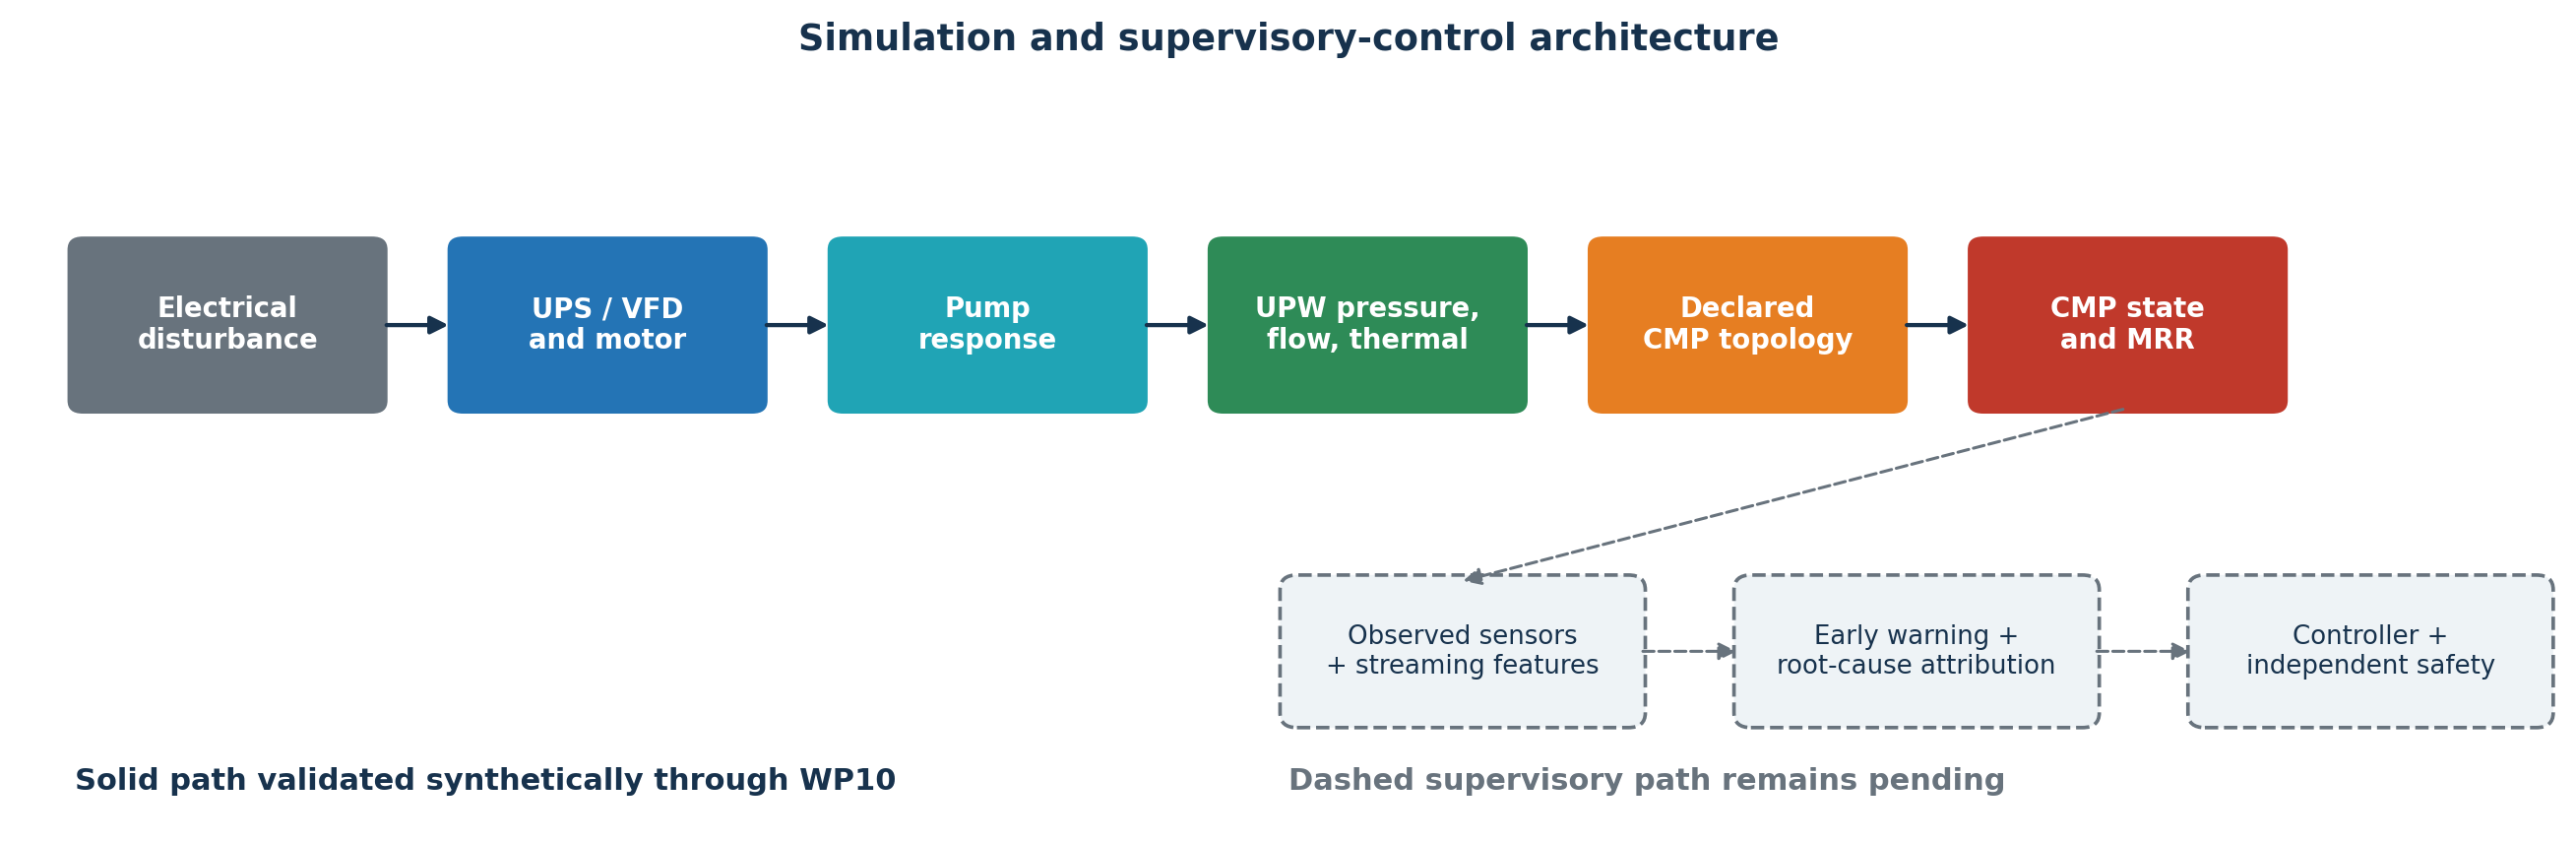
\includegraphics[width=0.94\textwidth]{system_architecture_wp10.png}
  \caption{Implemented synthetic propagation path through WP10 and the pending
  supervisory stages. Solid physical-state propagation is kept separate from
  observed sensor delivery and from later decision logic. The figure is
  generated from frozen repository artifacts; predictive-control results are
  not included.}
  \label{fig:architecture}
\end{figure*}

The sensor contract distinguishes three times:
\begin{equation}
\begin{aligned}
 t_{\mathrm{source}}&=t_k,\\
 t_{\mathrm{reported}}&=\max(0,t_{\mathrm{source}}
 +\epsilon_{\mathrm{clock}}),\\
 t_{\mathrm{arrival}}&=t_{\mathrm{source}}+d_{\mathrm{comm}}.
\end{aligned}
 \label{eq:clocks}
\end{equation}
Reported timestamp jitter does not alter the source or arrival time. At a
decision timestamp $t_d$, an online consumer may use only observations whose
$t_{\mathrm{arrival}}\leq t_d$, prior predictions and actions, and validated
static configuration. It may not use latent truth, future observations,
offline excursion labels, or simulator cause labels. Actions proposed at step
$k$ take effect no earlier than step $k+1$. Initiating scenario causes are
also kept distinct from downstream propagation states such as UPS transfer or
VFD derating.

\section{Reduced-order utility plant}

The utility model is deliberately lumped: it captures causal timing and
conservation at the proof-of-concept resolution, not switching waveforms,
distributed water hammer, detailed pump performance, or equipment protection.

\subsection{Electrical source, UPS, and drive}

Electrical scenarios prescribe bounded voltage and frequency events. The UPS
has explicit output voltage, output frequency, load, battery energy, transfer,
bypass, and recovery states. During battery or transfer operation, accepted
discharge follows
\begin{equation}
 E_b^{k+1}=E_b^k-\frac{P_L\Delta t}{\eta_{\mathrm{inv}}}.
 \label{eq:ups-energy}
\end{equation}
Depletion or overload moves the synthetic model to bypass rather than creating
energy. The VFD and motor use bounded commands, derating, slew limits, and
first-order speed dynamics. These are engineering approximations and not a
model of UPS electrochemistry, switching, protection relays, or motor
electromagnetics.

\subsection{Pump, hydraulic compliance, and thermal state}

Rather than determining flow and head independently from affinity rules, the
pump is solved against the network using the speed-scaled quadratic curve
\begin{equation}
\begin{aligned}
 H_p(Q,n,d)&=dH_{\mathrm{shut}}n^2-k_QQ^2,\\
 k_Q&=\frac{H_{\mathrm{shut}}-H_{\mathrm{ref}}}
 {Q_{\mathrm{ref}}^2},
\end{aligned}
 \label{eq:pump-curve}
\end{equation}
where $n$ is normalized speed and $d$ is a bounded degradation factor. A check
valve excludes reverse flow when network differential pressure exceeds shutoff
head. The supply node solves the implicit balance
\begin{equation}
\begin{aligned}
 \frac{C_h(P_s^{k+1}-P_s^k)}{\Delta t}
 &=Q_p^k-Q_t(P_s^{k+1})\\
 &\quad-Q_r(P_s^{k+1})-Q_{\mathrm{rel}}(P_s^{k+1}),
\end{aligned}
 \label{eq:hydraulic-balance}
\end{equation}
with tool, return, relief, and storage terms and without an after-the-fact
pressure clip. Every step audits the discrete mass residual. A well-mixed
thermal balance uses actual pump inflow. Water chemistry is not inferred; the
model emits only a dimensionless synthetic water-quality deviation index,
which has no CMP effect.

For a preregistered 0.70-pu speed case, a 10 ms hydraulic solution differs
from a 0.5 ms reference by 36.19 Pa, or 0.0121\% of nominal pressure. In a pump
trip, pressure falls from 300 to 290.244 kPa on the first step and then
decreases monotonically. Generated balance residuals remain below
$1.0\times10^{-12}$ m$^3$/s. These checks establish numerical behavior of the
synthetic equations, not manufacturer calibration.

\section{Reduced-order CMP subsystem}

\subsection{Modes and removal accounting}

The CMP state machine contains \textsc{idle}, \textsc{prepare},
\textsc{polish}, \textsc{dress}, \textsc{hold}, \textsc{recover}, and
\textsc{complete}. Let $\chi_p=1$ only during active polishing and
$\chi_d=1$ only during dressing. Material removal, cumulative active time,
and selected wear terms are mode-gated. A forced hold records an explicit
reason, and resumption requires 0.5 s of continuous valid recovery dwell in the
reference configuration. \textsc{complete} is terminal until reset.

The model records true instantaneous equivalent MRR $R_{\mathrm{true}}$,
cumulative removed thickness $H$, active polish time $t_p$, and active-time
average MRR:
\begin{equation}
 \dot H=R_{\mathrm{true}},\qquad
 \dot t_p=\chi_p,\qquad
 \overline R=\frac{H}{\max(t_p,\varepsilon)}.
 \label{eq:cumulative-removal}
\end{equation}
This accounting is essential for later control evaluation: holding the process
cannot appear beneficial merely because instantaneous MRR becomes zero.

\subsection{Signed rotary kinematics and exposure}

For platen angular velocity $\omega_p$, wafer angular velocity $\omega_w$,
center offset $r_{cc}$, and local wafer polar coordinate $(r,\theta)$, vector
subtraction gives
\begin{equation}
\begin{aligned}
 v_R(r,\theta)=\big[&\omega_p^2r_{cc}^2
 +(\omega_p-\omega_w)^2r^2\\
 &+2\omega_p(\omega_p-\omega_w)r_{cc}r\cos\theta
 \big]^{1/2}.
\end{aligned}
 \label{eq:relative-velocity}
\end{equation}
Angular velocities remain signed. Equal co-rotation produces the constant
field $|\omega_pr_{cc}|$, stopped axes produce zero, and counter-rotation
produces a nonuniform field. The normalized generalized-Preston exposure is
the contact-area mean
\begin{equation}
 \Phi_{PV}=\frac{1}{A}\int_A
 \left(\frac{p(r)}{P_0}\right)^{\alpha}
 \left(\frac{v_R(r,\theta)}{V_0}\right)^{\beta}\,\mathrm dA.
 \label{eq:exposure}
\end{equation}
The integral is evaluated by deterministic radial--angular quadrature. It is
not replaced with the product of average pressure and average speed because
that equality does not hold in general. The reported annular coefficient of
variation is only a \emph{simulated spatial-uniformity proxy; not
experimentally validated WIWNU}.

\subsection{Consumable memory and dressing}

The minimum consumable state comprises reversible pad-surface activity $g_p$,
irreversible remaining pad-life proxy $\ell_p$, and dresser effectiveness
$h_d$, each projected inside $[0,1]$. With dressing command $a_d$, the frozen
model structure is
\begin{align}
 \dot g_p &=-\chi_pk_g\Phi_{PV}g_p
 +\chi_dk_ca_dh_d(1-g_p), \label{eq:pad-activity}\\
 \dot\ell_p &=-\chi_pk_{wp}\Phi_{PV}-\chi_dk_{wd}a_d,\label{eq:pad-life}\\
 \dot h_d &=-\chi_dk_da_dh_d.\label{eq:dresser}
\end{align}
Dressing can restore reversible surface activity while consuming pad life and
dresser effectiveness. This separation prevents a conditioning action from
restoring an irreversible life state. The functional decomposition is
literature-informed \cite{borucki2002,borucki2004,chang2007,sun2010}; its rate
coefficients are synthetic assumptions.

\subsection{Slurry availability, interface temperature, and MRR}

A bounded dynamic availability state represents the recipe-selected slurry
line. The interface temperature $T_i$ is distinct from both slurry and UPW
temperature and follows the reduced balance
\begin{equation}
 C_i\dot T_i=\eta_f\mu A_cP_c\overline v_R
 -UA_T(T_i-T_c)-\rho_sc_{p,s}Q_s(T_i-T_s),
 \label{eq:thermal-balance}
\end{equation}
where the terms represent frictional input, coolant-boundary removal, and
slurry sensible-heat transport. The normalized equivalent removal rate is
\begin{equation}
 R_{\mathrm{eq}}=\chi_p R_{0,s}\Phi_{PV}
 m_s m_T m_{\mathrm{pad}}m_{\mathrm{recipe}},
 \label{eq:mrr}
\end{equation}
with dimensionless bounded slurry, temperature, pad, and recipe modifiers.
The default material profile fixes the temperature sensitivity at zero. Thus a
thermal boundary can change $T_i$ while having exactly zero effect on MRR; a
thermal-to-MRR effect requires a separately named non-null material profile.

For the classical $\alpha=\beta=1$ reference, pressure $P_0=30{,}000$ Pa,
platen/head speeds 8/6 rad/s, and power-mean speed
$V_0=1.6070416183328249$ m/s, the reference removal is
\begin{equation}
 R_0=1.6666666666667\times10^{-9}\ \mathrm{m/s}
 =100\ \mathrm{nm/min}.
\end{equation}
The corresponding derived Preston coefficient is
$K_P=3.4570078908840606\times10^{-14}$ Pa$^{-1}$, satisfying
$K_PP_0V_0=R_0$ to floating-point tolerance. The numerical values define the
synthetic reference recipe; they are not calibrated to the PHM target or a
real material stack.

\section{Typed utility-to-CMP coupling}

The coupler is stateless and consumes only latent UPW state. Its output is an
already defined typed CMP boundary. It cannot inspect raw voltage, UPS, VFD,
pump, or corrupted sensor fields; calculate MRR; inject a generic discrepancy
multiplier; force a hold; or take a control action.

For normalized pressure $p=P_s/P_{\mathrm{ref}}$ and tool flow
$q=Q_t/Q_{\mathrm{ref}}$, define the clipped ramp
\begin{equation}
 \mathcal R(x;x_0,x_1)=\operatorname{clip}
 \left(\frac{x-x_0}{x_1-x_0},0,1\right).
 \label{eq:ramp}
\end{equation}
Hydraulic support and link-adjusted availability are
\begin{equation}
\begin{aligned}
 a_h&=\min\{\mathcal R(p;p_0,p_1),
                 \mathcal R(q;q_0,q_1)\},\\
 a_{\mathrm{eff}}&=1-\lambda(1-a_h).
\end{aligned}
 \label{eq:availability}
\end{equation}
The minimum treats pressure and flow as correlated indicators of the same
hydraulic network and avoids multiplying the disturbance twice. The ramp,
minimum, and affine blend are engineering approximations; every numerical
threshold, reference, and link strength is a synthetic assumption.

The four frozen structures are:
\begin{description}
  \item[No connection:] exact neutral boundary and mandatory default.
  \item[Dressing-water support:] $a_{\mathrm{eff}}$ changes realized dressing
  availability only, allowing a delayed effect through Eq.~\eqref{eq:pad-activity}.
  \item[Thermal loop:] cooling conductance is scaled by
  $a_{\mathrm{eff}}$ and
  \begin{equation}
    T_c=T_{c,0}+\lambda(T_u-T_{u,\mathrm{ref}}).
    \label{eq:thermal-map}
  \end{equation}
  Neutral CMP and upstream temperatures are distinct, making zero link exactly
  neutral for any UPW temperature and nominal UPW temperature neutral for any
  link strength.
  \item[Synthetic slurry support:] $a_{\mathrm{eff}}$ changes only a
  specifically named synthetic slurry-utility availability boundary.
\end{description}

Nominal connected references are 300 kPa supply pressure and 100 mL/s tool
flow. Pressure zero/full fractions are 0.60/0.95, while flow zero/full
fractions are 0.50/0.95. These define the synthetic experiment and are not
operating limits for any real CMP tool. Every coupling parameter has a unit,
hard bound, sensitivity range, expected direction, and provenance class.

\section{Validation design}

The scientific checks cover dimensions, limiting cases, monotonicity, state
bounds, process-mode gating, energy and mass residuals, deterministic replay,
quadrature convergence, timestep refinement, null topologies, and parameter
mismatch. Two full-chain cases serve different purposes.

The negative control is a 25\% voltage sag lasting 400 ms with a healthy UPS.
It asks whether the coupling remains inactive when the synthetic utility plant
rides through the event. The positive chain is separately configured as a
degraded 500 J UPS with 2,500 W load, 0.95 inverter efficiency, a grid
interruption from 1 to 4 s during a 6 s dressing interval, and an explicit VFD
restart request. A 1 s preparation interval follows and polishing starts at
7 s. The connected and no-connection runs share identical upstream states,
initial conditions, timestep, and disturbance.

Local derivatives are evaluated only away from ramp and minimum knots. Global
sensitivity uses seeded Saltelli pick--freeze Monte Carlo estimators
\cite{saltelli2010}: 4,096 base samples, seven independent parameter ranges,
seed 20260711, and 36,864 evaluations at one representative degraded state.
Raw finite-sample indices are retained without clipping or renormalization.
Structural and mismatch cases include no connection, zero link, several link
strengths, and earlier- and later-response thresholds.

\section{Results through WP10}

All numerical results in this section are \simonly{} and conditional on the
specified configuration. The public-data archive evidence in
Section~4 is provenance and schema evidence, not a public-model performance
result.

\subsection{Standalone CMP invariants and reference trace}

The $16\times64$ radial--angular quadrature gives
$V_0=1.6070416183328249$ m/s. Nominal exposure differs from one only at
floating-point precision, and both zero pressure and zero speed produce
exactly zero exposure and removal. Across $8\times32$, $16\times64$,
$32\times128$, and $48\times192$ grids, the constant-field integral differs
from one by at most $2.22\times10^{-16}$ and nominal area-mean velocity differs
from the finest grid by at most $4.44\times10^{-16}$ m/s.

The nominal annular exposure coefficient of variation is
0.0025316618572622336. This is a \emph{simulated spatial-uniformity proxy; not
experimentally validated WIWNU}.

\begin{figure}[t]
  \centering
  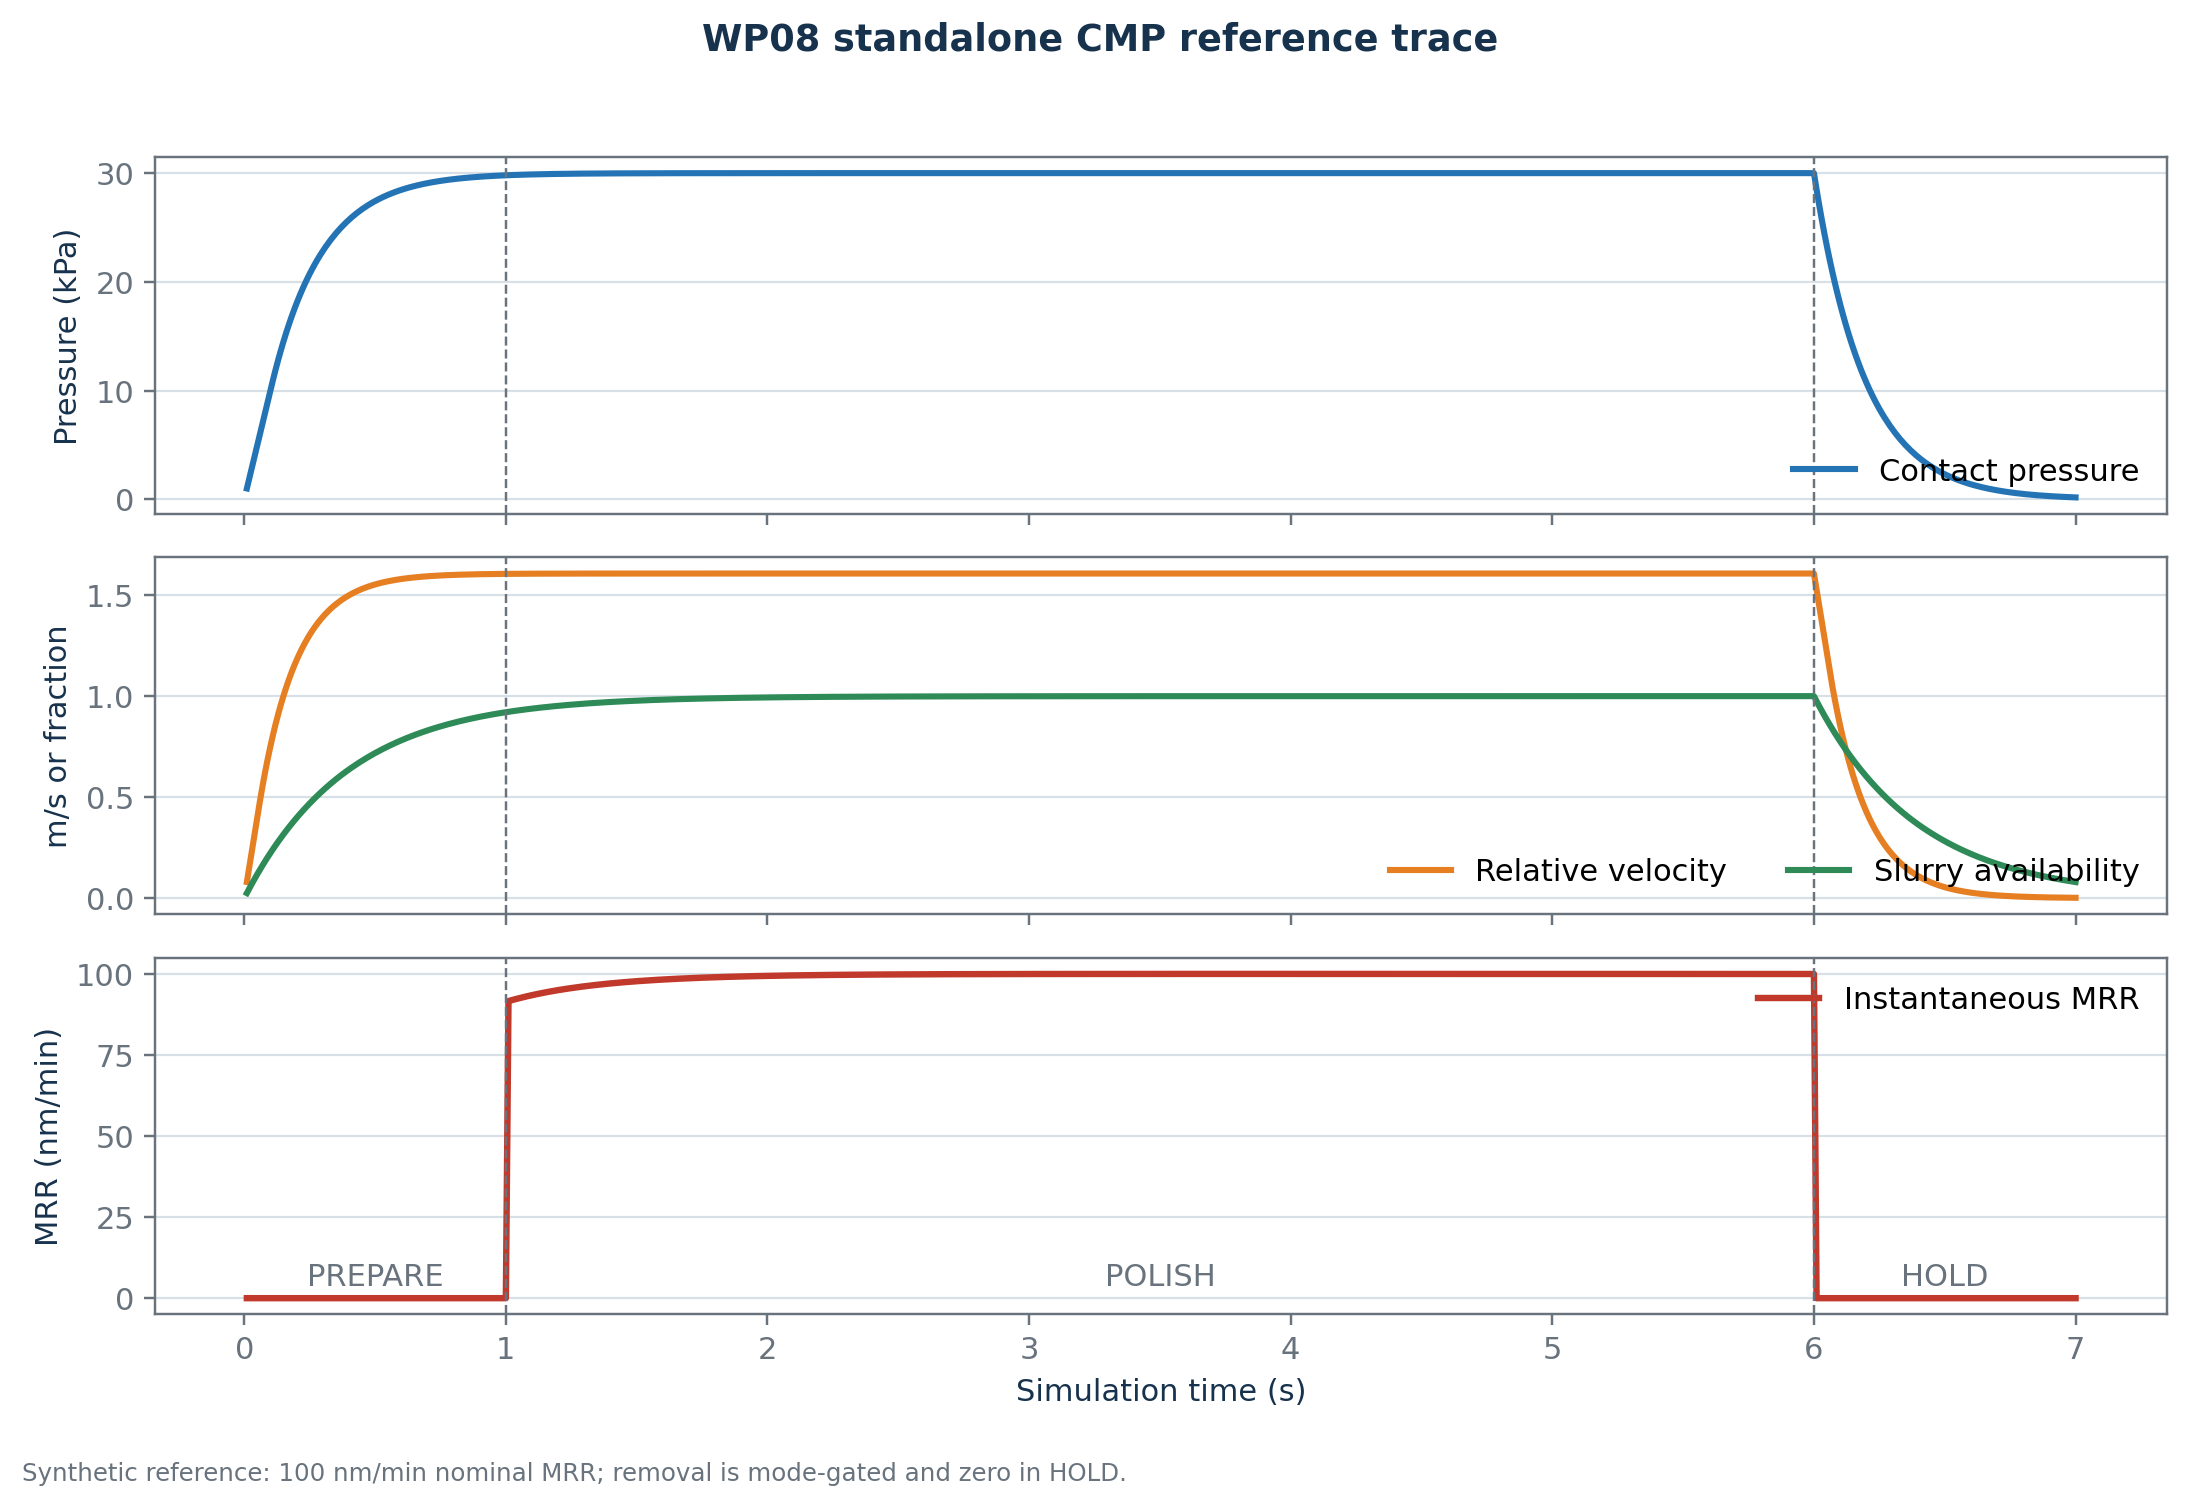
\includegraphics[width=\columnwidth]{wp08_reference_trace.png}
  \caption{Frozen WP08 synthetic reference trace. Material removal is gated
  to \textsc{polish}; cumulative removal and active-time average retain process
  history across non-polishing modes.}
  \label{fig:wp08-trace}
\end{figure}

Figure~\ref{fig:wp08-trace} contains 1 s \textsc{prepare}, 5 s
\textsc{polish}, and 1 s \textsc{hold} at a 10 ms step. Only polishing
increases active time and cumulative removal. Final active time is
4.999999999999938 s, cumulative removal is
$8.276153498157771\times10^{-9}$ m, and active-time average MRR is
$1.6552306996315749\times10^{-9}$ m/s. The average is below the fresh-pad
100 nm/min reference because pad activity decays during polishing.

A separate 10 s dressing limit starts at pad activity 0.5, remaining pad life
0.8, and dresser effectiveness 0.9. It ends at 0.5823912561, 0.7995, and
0.8998200179, respectively, with exactly zero instantaneous MRR. The case
confirms restoration of reversible surface activity without restoration of
remaining life.

The maximum absolute discrete interface-energy residual over the 700-step
reference is $1.4188941577231162\times10^{-8}$ W, below the
$10^{-7}$ W audit tolerance. With default thermal sensitivity zero, cold and
warm coolant boundaries produce different temperatures after 1 s but exactly
zero instantaneous-MRR difference.

Table~\ref{tab:timestep} reports refinement of a 70\% pressure-command case
against a 1 ms reference. All three error measures decrease monotonically,
supporting the 10 ms default within the tested standalone configuration.

\begin{table}[t]
\centering
\caption{Standalone CMP timestep refinement.}
\label{tab:timestep}
\small
\begin{tabular}{rrrr}
\toprule
$\Delta t$ & $|e_P|$ & $|e_T|$ & $|e_H|$\\
(s) & (Pa) & (K) & (m)\\
\midrule
0.0400 & 25.8847 & $2.8404\times10^{-4}$ & $1.9141\times10^{-11}$\\
0.0200 & 13.5017 & $1.3801\times10^{-4}$ & $9.3021\times10^{-12}$\\
0.0100 &  6.6010 & $6.5280\times10^{-5}$ & $4.4005\times10^{-12}$\\
0.0050 &  2.9787 & $2.8992\times10^{-5}$ & $1.9545\times10^{-12}$\\
0.0025 &  1.1254 & $1.0868\times10^{-5}$ & $7.3269\times10^{-13}$\\
\bottomrule
\end{tabular}
\end{table}

At the WP08 evidence freeze, 48 focused CMP/contract checks and all 130
repository tests passed. This test evidence supports the declared synthetic
structure and numerics only.

\subsection{Healthy-sag negative control}

The healthy-UPS 25\%, 400 ms sag is replayed after 3 s plant warm-up, followed
by 6 s of dressing, 1 s preparation, and polishing from 7 s. Minimum UPS
output is 0.865536 pu; minimum motor speed is 187.1656743 rad/s; minimum pump
flow is $1.9724375\times10^{-4}$ m$^3$/s; and minimum supply pressure is
298.8797567 kPa. Tool flow remains 100 mL/s. Both hydraulic and effective
support remain exactly one.

\begin{figure}[t]
  \centering
  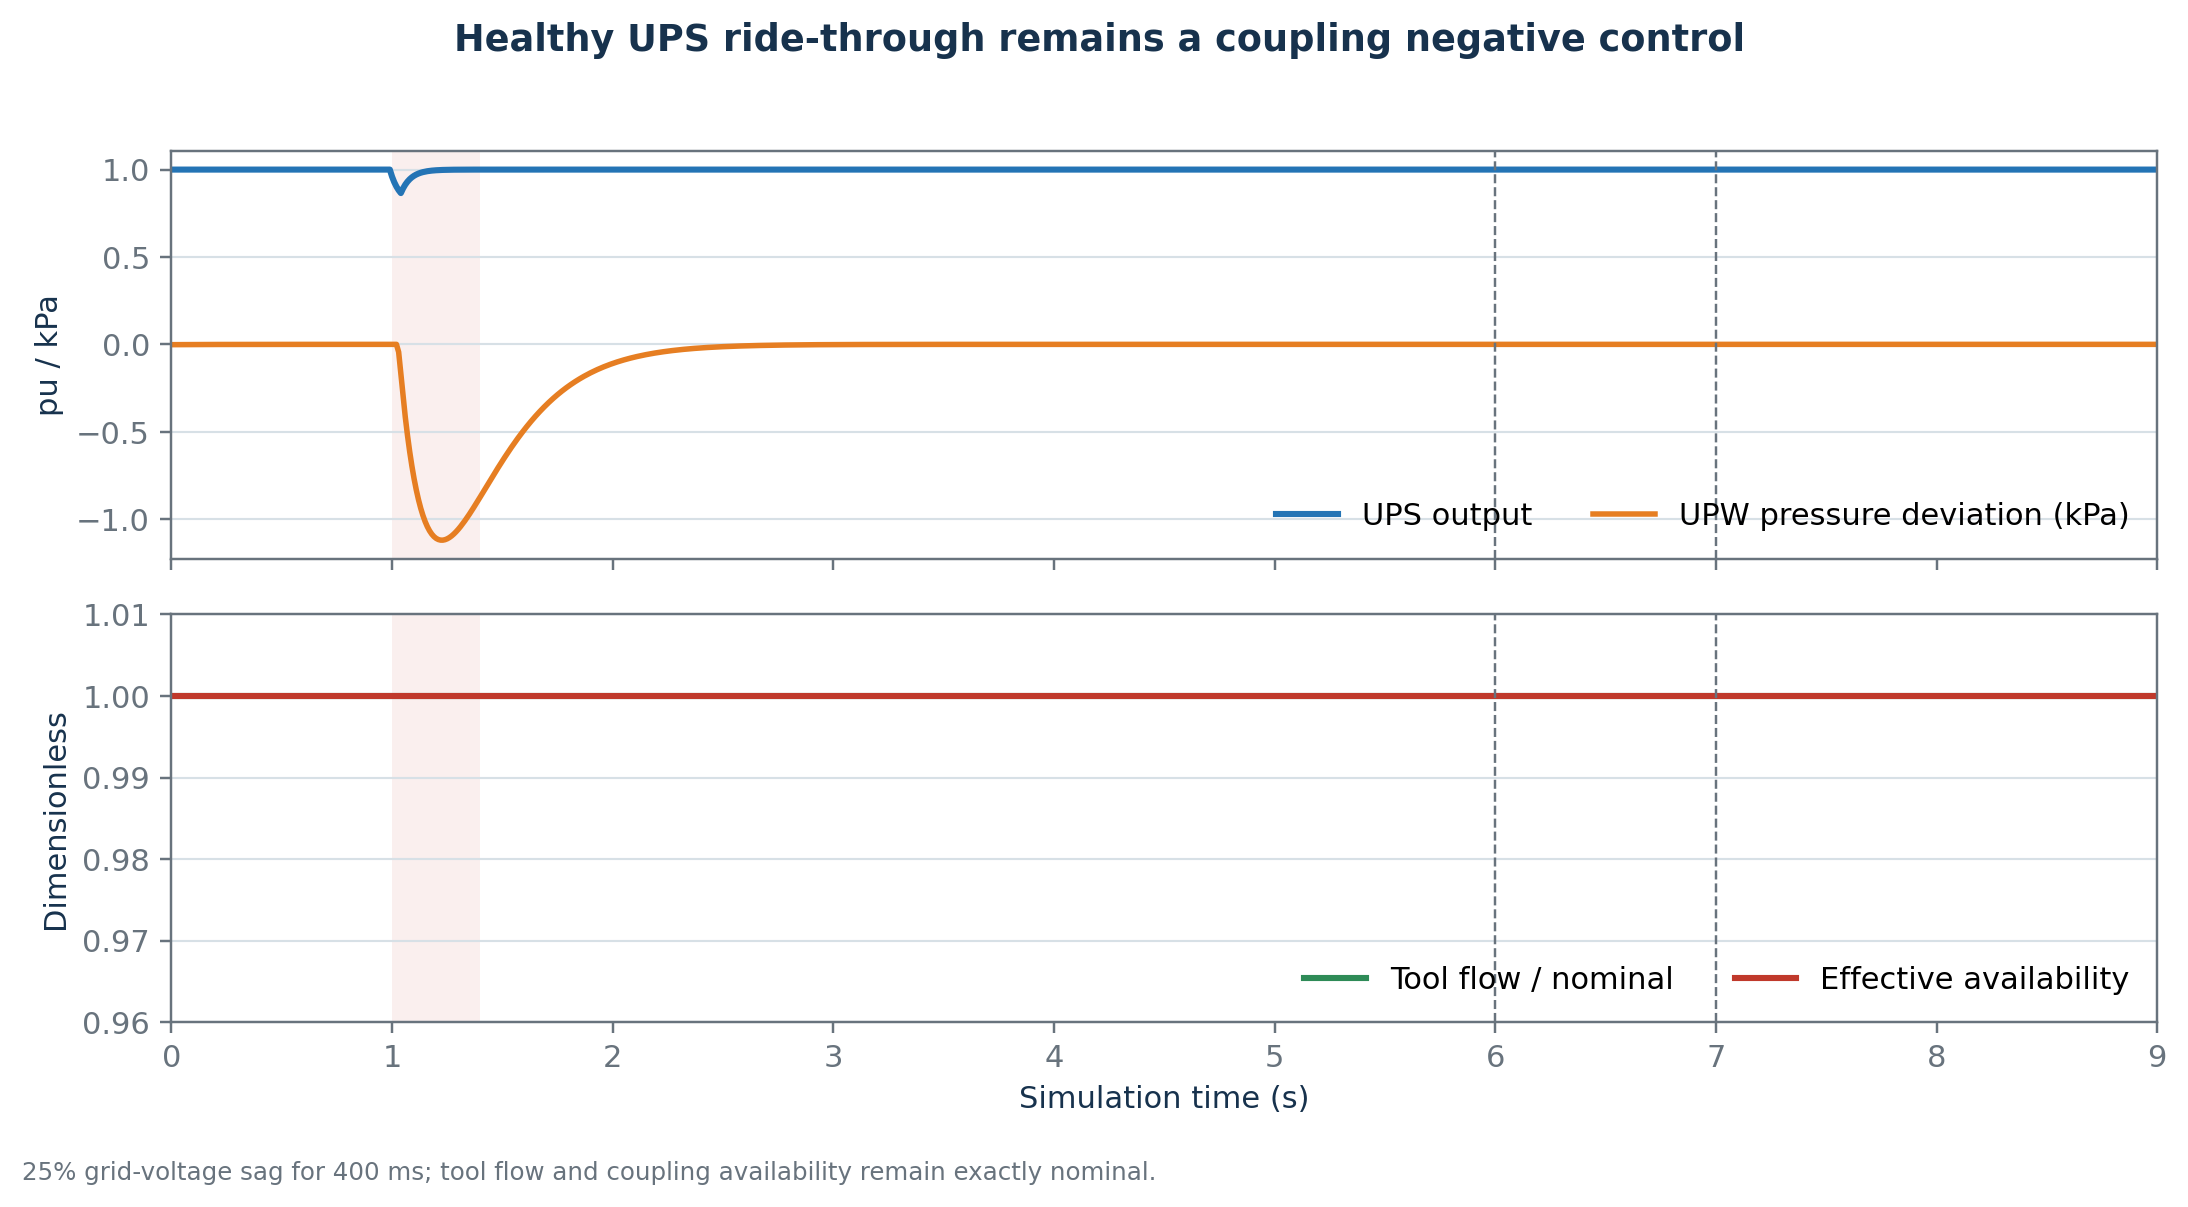
\includegraphics[width=\columnwidth]{wp10_negative_control.png}
  \caption{Healthy-UPS synthetic negative control. The electrical sag changes
  upstream states slightly, but the declared dressing-water connection remains
  at full support and connected/no-connection CMP traces are identical.}
  \label{fig:negative}
\end{figure}

As shown in Fig.~\ref{fig:negative}, connected and no-connection upstream
traces are identical by construction, and their pad activity, MRR, and
cumulative-removal traces also match exactly. The connected trace SHA-256 is
\texttt{f8359518\ldots bfc3f20}. This result is a structural negative control,
not a failed attempt to force an excursion: the coupling was not tuned to turn
a well-ridden-through event into a CMP perturbation.

\subsection{Declared positive causal chain}

The positive synthetic stress case produces the ordered onsets in
Table~\ref{tab:onsets}. The minimum UPS output approaches zero, pump flow
reaches zero, supply pressure approaches the 100 kPa return boundary, tool
flow approaches zero, and dressing availability reaches zero. Upstream traces
remain identical between the connected and no-connection variants.

\begin{table}[t]
\centering
\caption{First source-time onsets in the positive synthetic chain.}
\label{tab:onsets}
\small
\begin{tabular}{lr}
\toprule
Event & Time (s)\\
\midrule
Grid interruption & 1.00\\
UPS output $<0.9$ pu & 1.03\\
Pump flow $<99\%$ reference & 1.04\\
Motor speed $<99\%$ nominal & 1.19\\
UPW pressure below full support & 1.24\\
Effective availability $<1$ & 1.24\\
Polishing starts & 7.00\\
\bottomrule
\end{tabular}
\end{table}

\begin{figure*}[t]
  \centering
  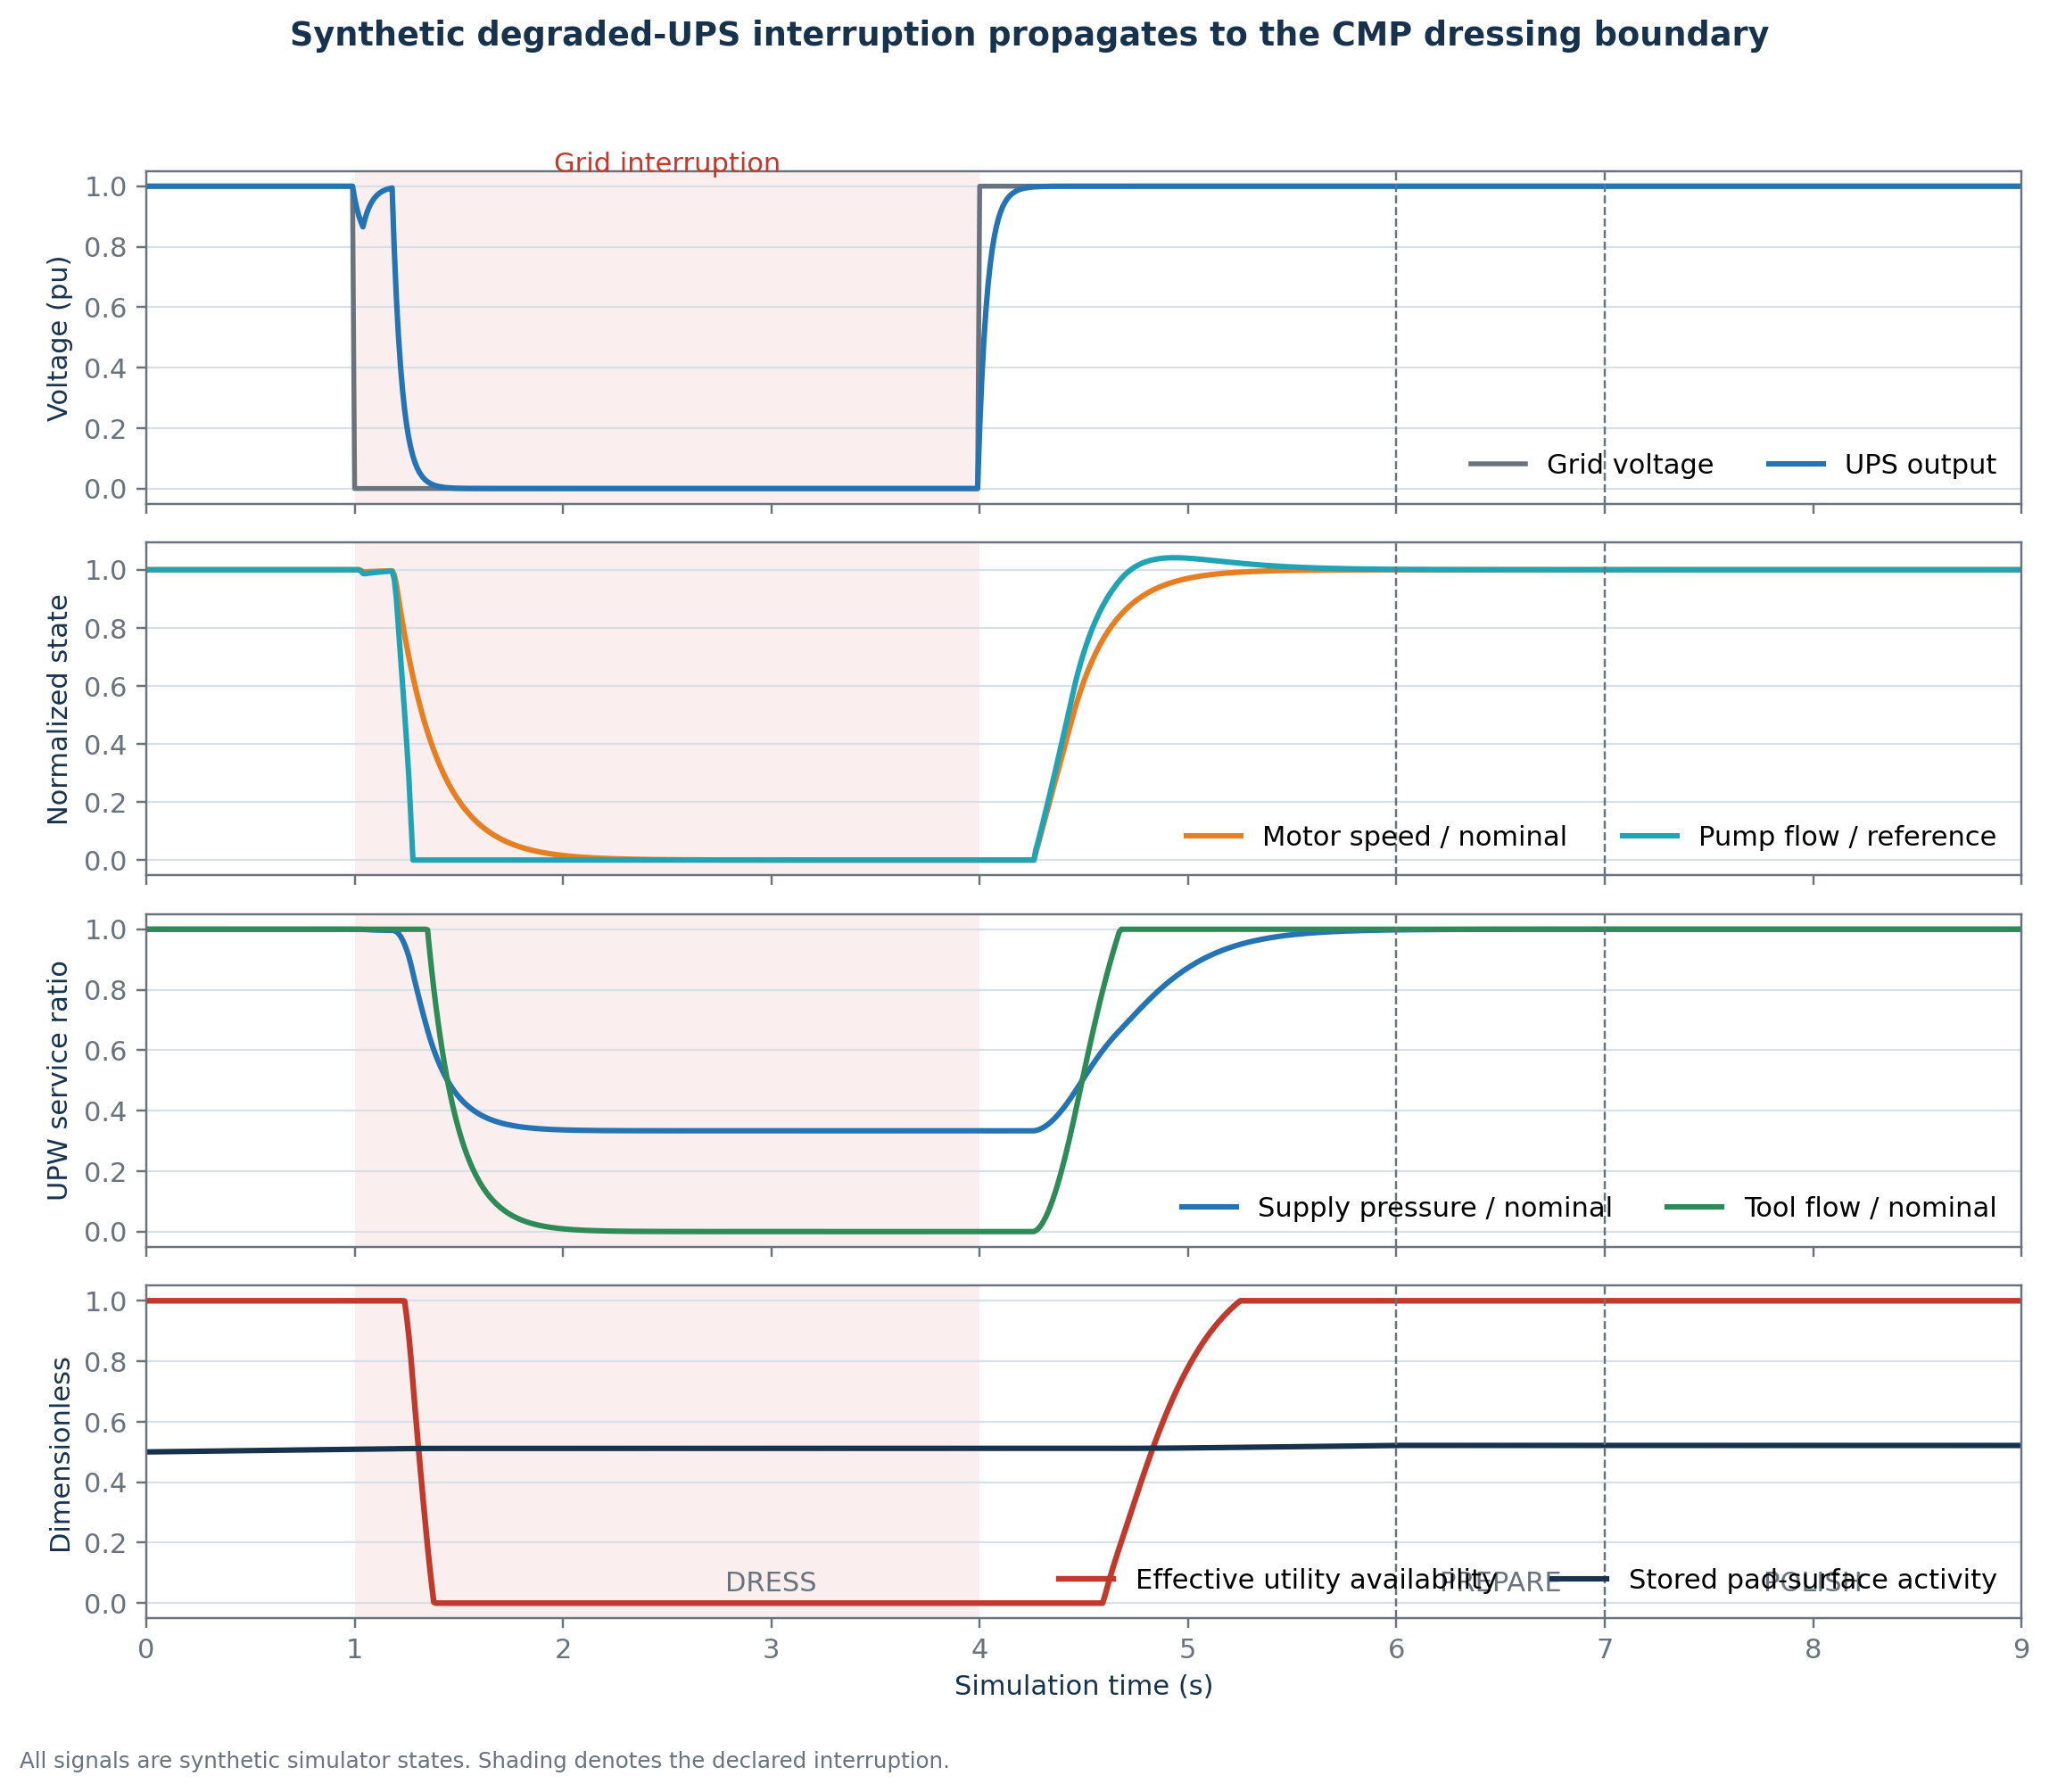
\includegraphics[width=0.90\textwidth]{wp10_positive_chain.png}
  \caption{Positive synthetic full-chain stress test. A deliberately degraded
  UPS during \textsc{dress} propagates through the drive, pump, and UPW state
  to dressing availability. This experiment is not a real UPS specification
  or real-tool plumbing model.}
  \label{fig:positive-chain}
\end{figure*}

The connected boundary affects only dressing availability. Therefore MRR is
exactly zero during dressing in both variants. By the end of dressing, pad
activity is 0.5511876609 with no connection and 0.5216572820 with
dressing-water support, a 5.3576\% relative decrease. When polishing begins
after utility recovery, the stored pad difference changes later removal
(Table~\ref{tab:positive-result} and Fig.~\ref{fig:delayed-result}).

\begin{table*}[t]
\centering
\caption{Positive synthetic chain result. Values are paired against identical
upstream states; no safe envelope or controller is involved.}
\label{tab:positive-result}
\small
\begin{tabular}{lrrr}
\toprule
Metric & No connection & Dressing-water support & Relative decrease\\
\midrule
End-of-dress pad activity & 0.5511876609 & 0.5216572820 & 5.3576\%\\
Mean later-polish MRR (m/s) & $1.0198314108\times10^{-9}$ & $9.8727270376\times10^{-10}$ & 3.1926\%\\
Final cumulative removal (m) & $2.0396628215\times10^{-9}$ & $1.9745454075\times10^{-9}$ & 3.1926\%\\
\bottomrule
\end{tabular}
\end{table*}

\begin{figure*}[t]
  \centering
  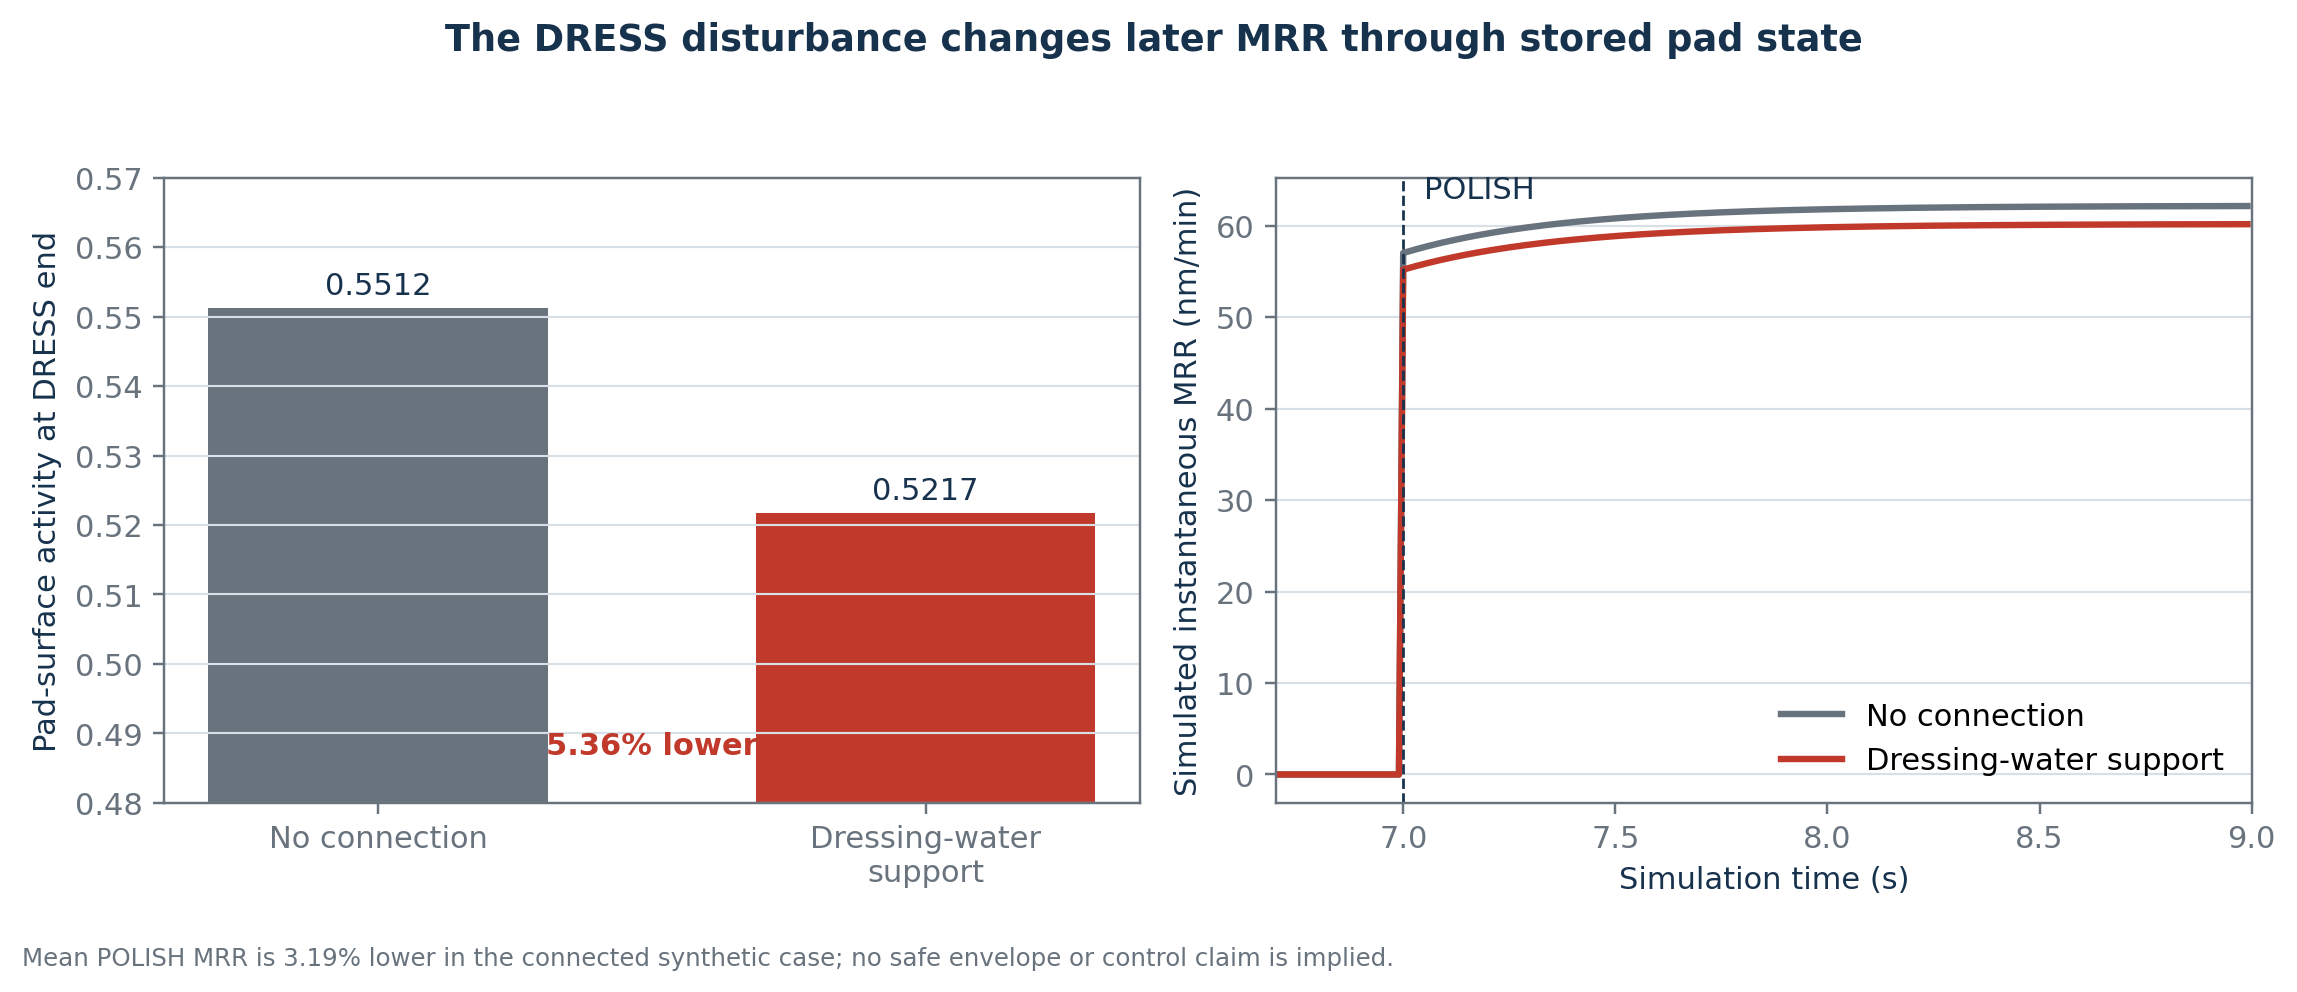
\includegraphics[width=0.82\textwidth]{wp10_delayed_mrr_result.png}
  \caption{Delayed synthetic CMP result. Utility support changes pad activity
  during \textsc{dress}; only later, during \textsc{polish}, does MRR differ.
  There is no direct instantaneous UPW-to-MRR multiplier.}
  \label{fig:delayed-result}
\end{figure*}

The positive no-connection and connected trace SHA-256 values are
\texttt{3560cb28\ldots 41fc3f20} and
\texttt{19f440b2\ldots 51dfa10}, respectively. The delayed 3.1926\% effect is
conditional on the selected synthetic topology and values; it is neither a
safe-envelope violation nor evidence of controller benefit.

\subsection{Sensitivity and structural uncertainty}

Off-knot finite-difference signs match the frozen expectations. Increasing
link strength, reference pressure or flow, or the transition thresholds
reduces availability at their selected transition states. In the 0.5-link
thermal case, increasing the UPW reference temperature changes mapped coolant
temperature with derivative $-0.5$. Derivatives at ramp and minimum knots are
deliberately not reported.

\begin{figure}[t]
  \centering
  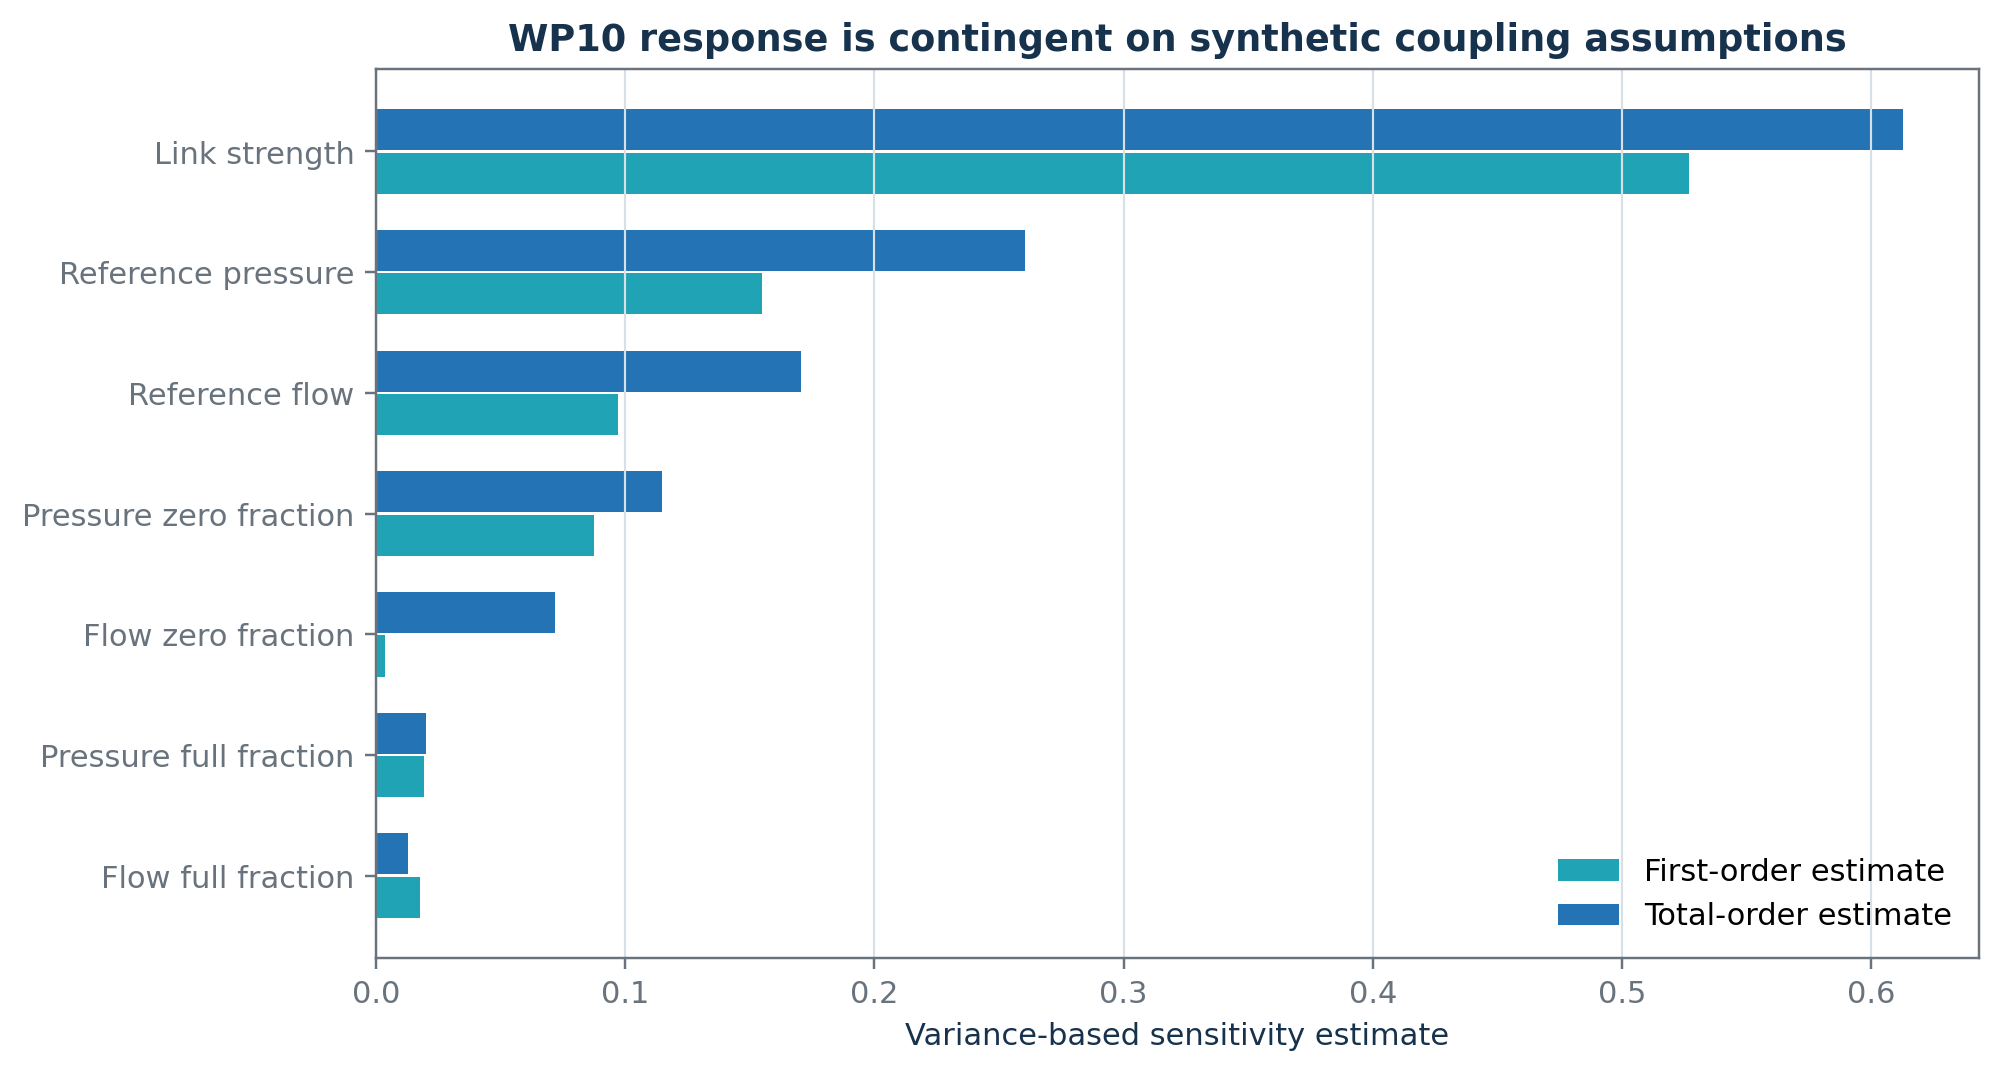
\includegraphics[width=\columnwidth]{wp10_global_sensitivity.png}
  \caption{Raw Saltelli first- and total-order estimates for effective
  availability at one representative degraded state. These are conditional
  simulator sensitivities, not empirical feature importance or causal proof.}
  \label{fig:sensitivity}
\end{figure}

\begin{table*}[t]
\centering
\caption{Seeded global sensitivity of effective availability. Raw estimates
are conditional on the chosen state, ranges, topology, and output.}
\label{tab:sensitivity}
\small
\begin{tabular}{lrrl}
\toprule
Parameter & First order & Total order & Sampled range\\
\midrule
Link strength & 0.5268 & 0.6127 & $[0,1]$\\
Reference supply pressure (Pa) & 0.1551 & 0.2603 & $[250{,}000,350{,}000]$\\
Pressure zero fraction & 0.0875 & 0.1147 & $[0.40,0.75]$\\
Pressure full fraction & 0.0194 & 0.0201 & $[0.85,1.00]$\\
Reference tool flow (m$^3$/s) & 0.0971 & 0.1705 & $[8\times10^{-5},1.2\times10^{-4}]$\\
Flow zero fraction & 0.0038 & 0.0718 & $[0.30,0.70]$\\
Flow full fraction & 0.0178 & 0.0128 & $[0.85,1.00]$\\
\bottomrule
\end{tabular}
\end{table*}

Figure~\ref{fig:sensitivity} and Table~\ref{tab:sensitivity} show that link
strength and reference pressure dominate this selected analysis. A small
first-/total-order inconsistency for the flow-full fraction is preserved as a
finite-sample estimator result, rather than corrected cosmetically. Across
zero, 0.25, and 1.0 link strengths and alternate threshold sets, mean later MRR
spans $9.8585309520\times10^{-10}$ to
$1.0198314108\times10^{-9}$ m/s. Zero link exactly matches no connection. The
simulated effect is therefore materially contingent on structure and parameter
assumptions.

At the WP10 evidence freeze, all 50 coupling-impacted tests and all 154
repository tests passed. The runtime schema/interface versions are
2.4.0/3.2.0 and the default topology remains no connection with link strength
zero. Test counts certify the checked software contracts and synthetic
invariants, not real-fab validity.

\section{Virtual-metrology and early-warning results; remaining protocols}

WP09 is now a frozen offline public-data result and WP12 a frozen synthetic
early-warning result. The attribution, control, safety, and integrated-runtime
subsections remain protocols so that modelling and evaluation choices are
fixed before their results are inspected. The WP12 runner is open loop: it does
not propose or apply controller actions and is not the WP17 runtime.

\subsection{WP09: public-data virtual metrology}

The one-shot WP09 study compares a training-target mean, ordinary linear and
ridge regression, a dimensionless native-scale physics proxy, histogram
gradient boosting, and a physics-plus-residual tree. All scientific choices,
the 405-column predictor order, whole-wafer roles, and interpretation gates
were committed before official holdout targets were opened. Training wafers
were assigned by feature identity to TRAIN\_CORE (1,396 rows/1,189 wafers),
MODEL\_SELECTION (299/255), and INTERVAL\_CALIBRATION (286/255). Five grouped
folds inside TRAIN\_CORE tune hyperparameters; MODEL\_SELECTION recommends a
family; final development fitting combines the first two roles; and the third
supplies interval scores. The retained test/final-validation roles contain
311/275 rows from 302/267 additional whole wafers.

For six active-polish proxy pressures, fit-only positive medians $m_j^+$ give
$P_i^*=\frac{1}{6}\sum_j\max(0,p_{ij})/m_j^+$. Absolute wafer, stage, and
head rotations are similarly normalized, with
$V_i^*=(\max(r_{w,i}^*,r_{s,i}^*)+r_{h,i}^*)/2$. The declared exposure and
native coefficient are
\begin{equation}
 \begin{aligned}
 \phi_i &={} \mathbb I[\text{active support}]P_i^*V_i^*,\\
 \widehat K_{native} &={} \max\left(0,
 \frac{\sum_i\phi_i y_i}{\sum_i\phi_i^2}\right).
 \end{aligned}
 \label{eq:wp09-native-proxy}
\end{equation}
This is not an SI Preston coefficient. The hybrid predicts
$\max(0,\widehat K_{native}\phi_i+f_\theta(X_i))$. Common fit-only median
imputation appends one missing indicator per predictor and removes
zero-variance derived columns. Linear/ridge designs are standardized; tree
designs are not. No target-driven feature selection occurs.

For calibration residuals $s_i=|y_i-\widehat y_i|$, the symmetric 90\%
split-conformal radius uses
\begin{equation}
 \begin{aligned}
 k &={} \min\{n,\lceil(n+1)(1-0.10)\rceil\},\\
 q &={} s_{(k)},\\
 [L_i,U_i] &={} [\max(0,\widehat y_i-q),\widehat y_i+q].
 \end{aligned}
 \label{eq:wp09-conformal}
\end{equation}
The selected tree uses absolute loss, 15 leaves, minimum leaf size 20, L2
regularization 0.1, and radius $q=5.3498$ in the source-native target scale.

\begin{table*}[t]
\centering
\caption{WP09 primary precedence-retained holdout results. Target values are
source-native and the unit is undeclared. Coverage is empirical for the
nominal 90\% split-conformal interval.}
\label{tab:wp09-primary}
\scriptsize
\begin{tabular}{lrrrrrrc}
\toprule
Family & Test MAE & Val. MAE & Test RMSE & Val. RMSE & Test $R^2$ & Val. $R^2$ & Test/val. coverage\\
\midrule
Mean & 29.540 & 29.703 & 33.152 & 33.170 & -0.022 & -0.020 & 0.852/0.865\\
Linear & 101.255 & 215.637 & 413.773 & 1955.543 & -158.132 & -3542.915 & 0.894/0.895\\
Ridge & 28.426 & 35.325 & 47.449 & 65.038 & -1.093 & -2.920 & 0.913/0.884\\
Physics proxy & 34.077 & 35.709 & 61.086 & 62.124 & -2.468 & -2.577 & 0.875/0.887\\
\textbf{Tree} & \textbf{3.185} & \textbf{3.395} & \textbf{5.176} & \textbf{6.693} & \textbf{0.975} & \textbf{0.958} & \textbf{0.839/0.847}\\
Hybrid & 4.723 & 5.935 & 8.251 & 11.704 & 0.937 & 0.873 & 0.916/0.905\\
\bottomrule
\end{tabular}
\end{table*}

The tree was recommended on MODEL\_SELECTION before holdout access and reduces
MAE relative to the mean by 89.22\%/88.57\%. The final-validation whole-wafer
bootstrap interval for paired tree-minus-mean MAE is
$[-28.191,-24.363]$, so the preregistered public-prediction gate passes. Its
test/final-validation grouped-bootstrap MAE intervals are
$[2.779,3.737]$ and $[2.784,4.108]$. Relative MAE is 3.572\%/3.858\%.

The hybrid is worse than the tree on both roles; the final-validation paired
hybrid-minus-tree interval is $[1.502,3.650]$. Thus the physics-plus-residual
improvement claim fails. Ordinary least squares has severe extrapolation and
22/23 clipped negative predictions on test/validation. The physics proxy is
also worse than the mean in MAE; it remains a structural baseline rather than
a calibrated physical model.

\begin{figure*}[t]
\centering
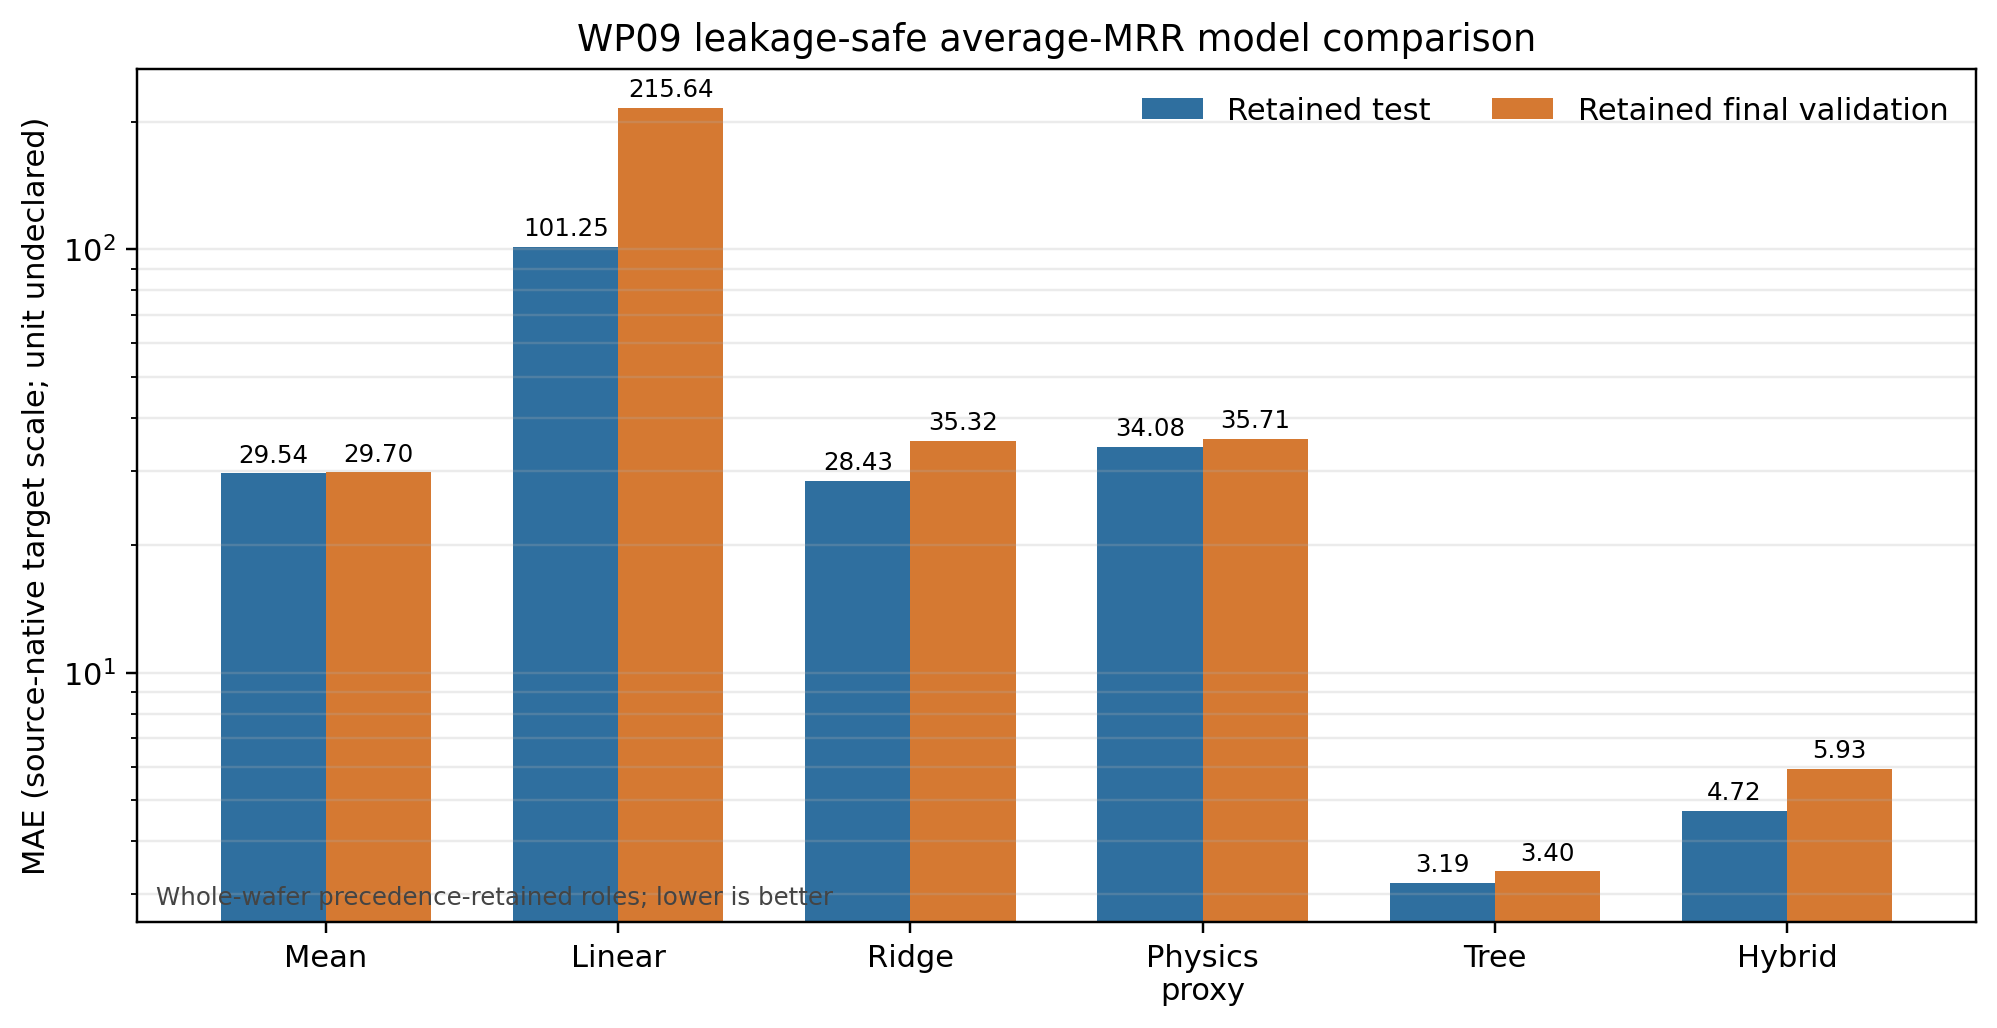
\includegraphics[width=0.48\textwidth]{wp09_model_comparison.png}\hfill
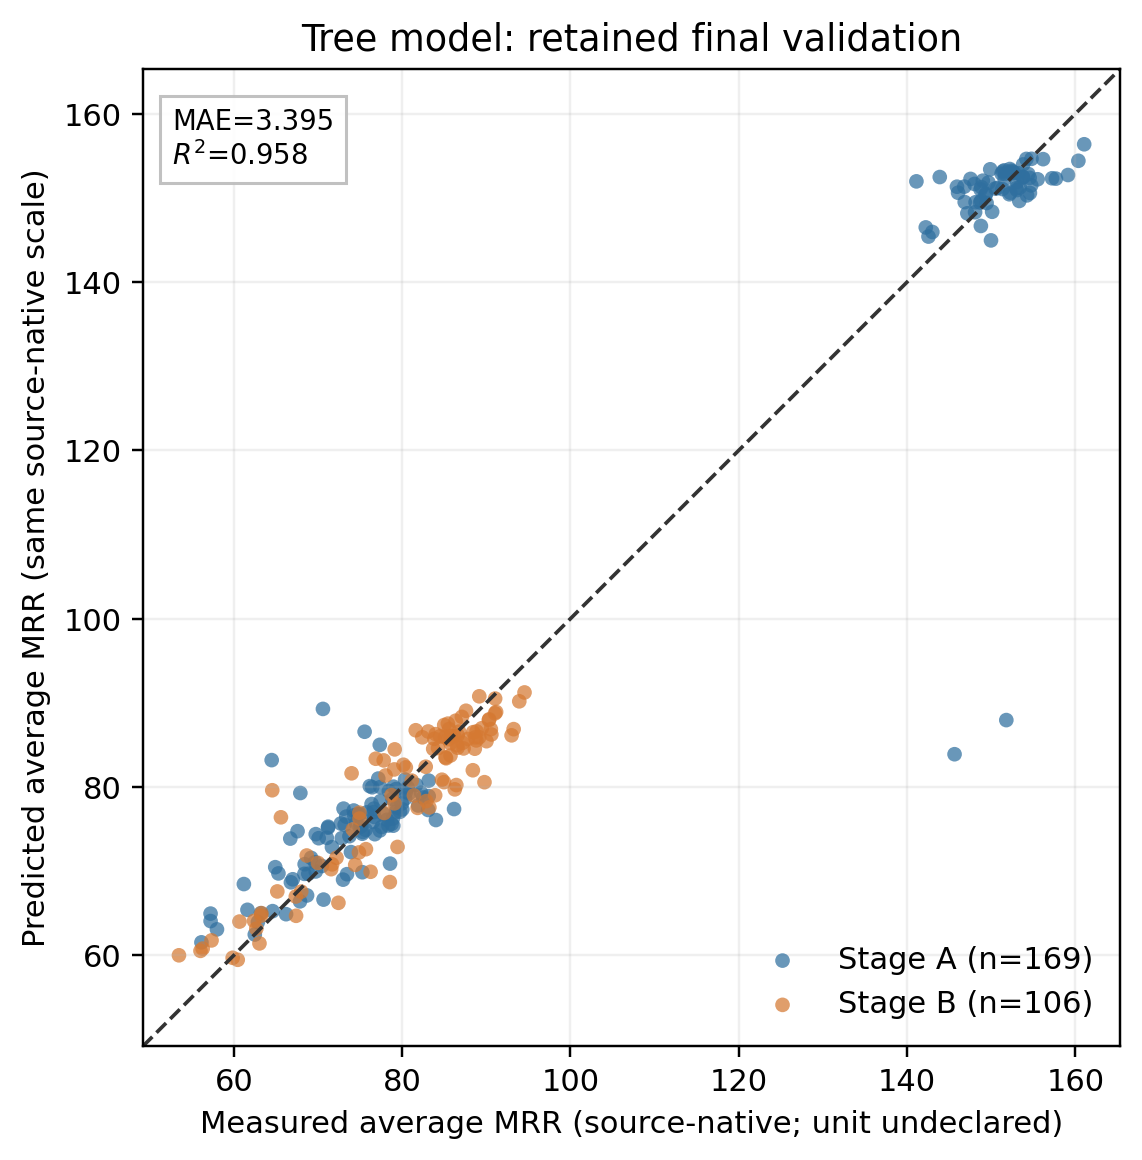
\includegraphics[width=0.39\textwidth]{wp09_tree_validation_scatter.png}
\caption{WP09 public-data results in the source-native target scale. Left: all
six frozen model families on mutually whole-wafer-disjoint retained roles; the
MAE axis is logarithmic. Right: tree predictions on retained final validation,
stratified by source stage. Neither axis has a declared physical unit.}
\label{fig:wp09-primary}
\end{figure*}

The primary tree intervals fail the frozen 0.85 coverage floor on both roles.
Test Stage A/B coverage is 0.853/0.818 and validation coverage 0.852/0.840, so
the shortfall is not isolated to one role. Gap-threshold (5/20 s), active-only,
and no-unresolved-proxy sensitivities keep tree MAE near 3.0--3.6 and generally
increase coverage, but secondary variants cannot rescue the primary gate.
Excluding the four preregistered extreme training labels yields MAE
3.050/3.100; the separately labelled hypothetical divide-by-60 sensitivity
yields 3.032/3.356. The original-label result remains primary.

\begin{figure*}[t]
\centering
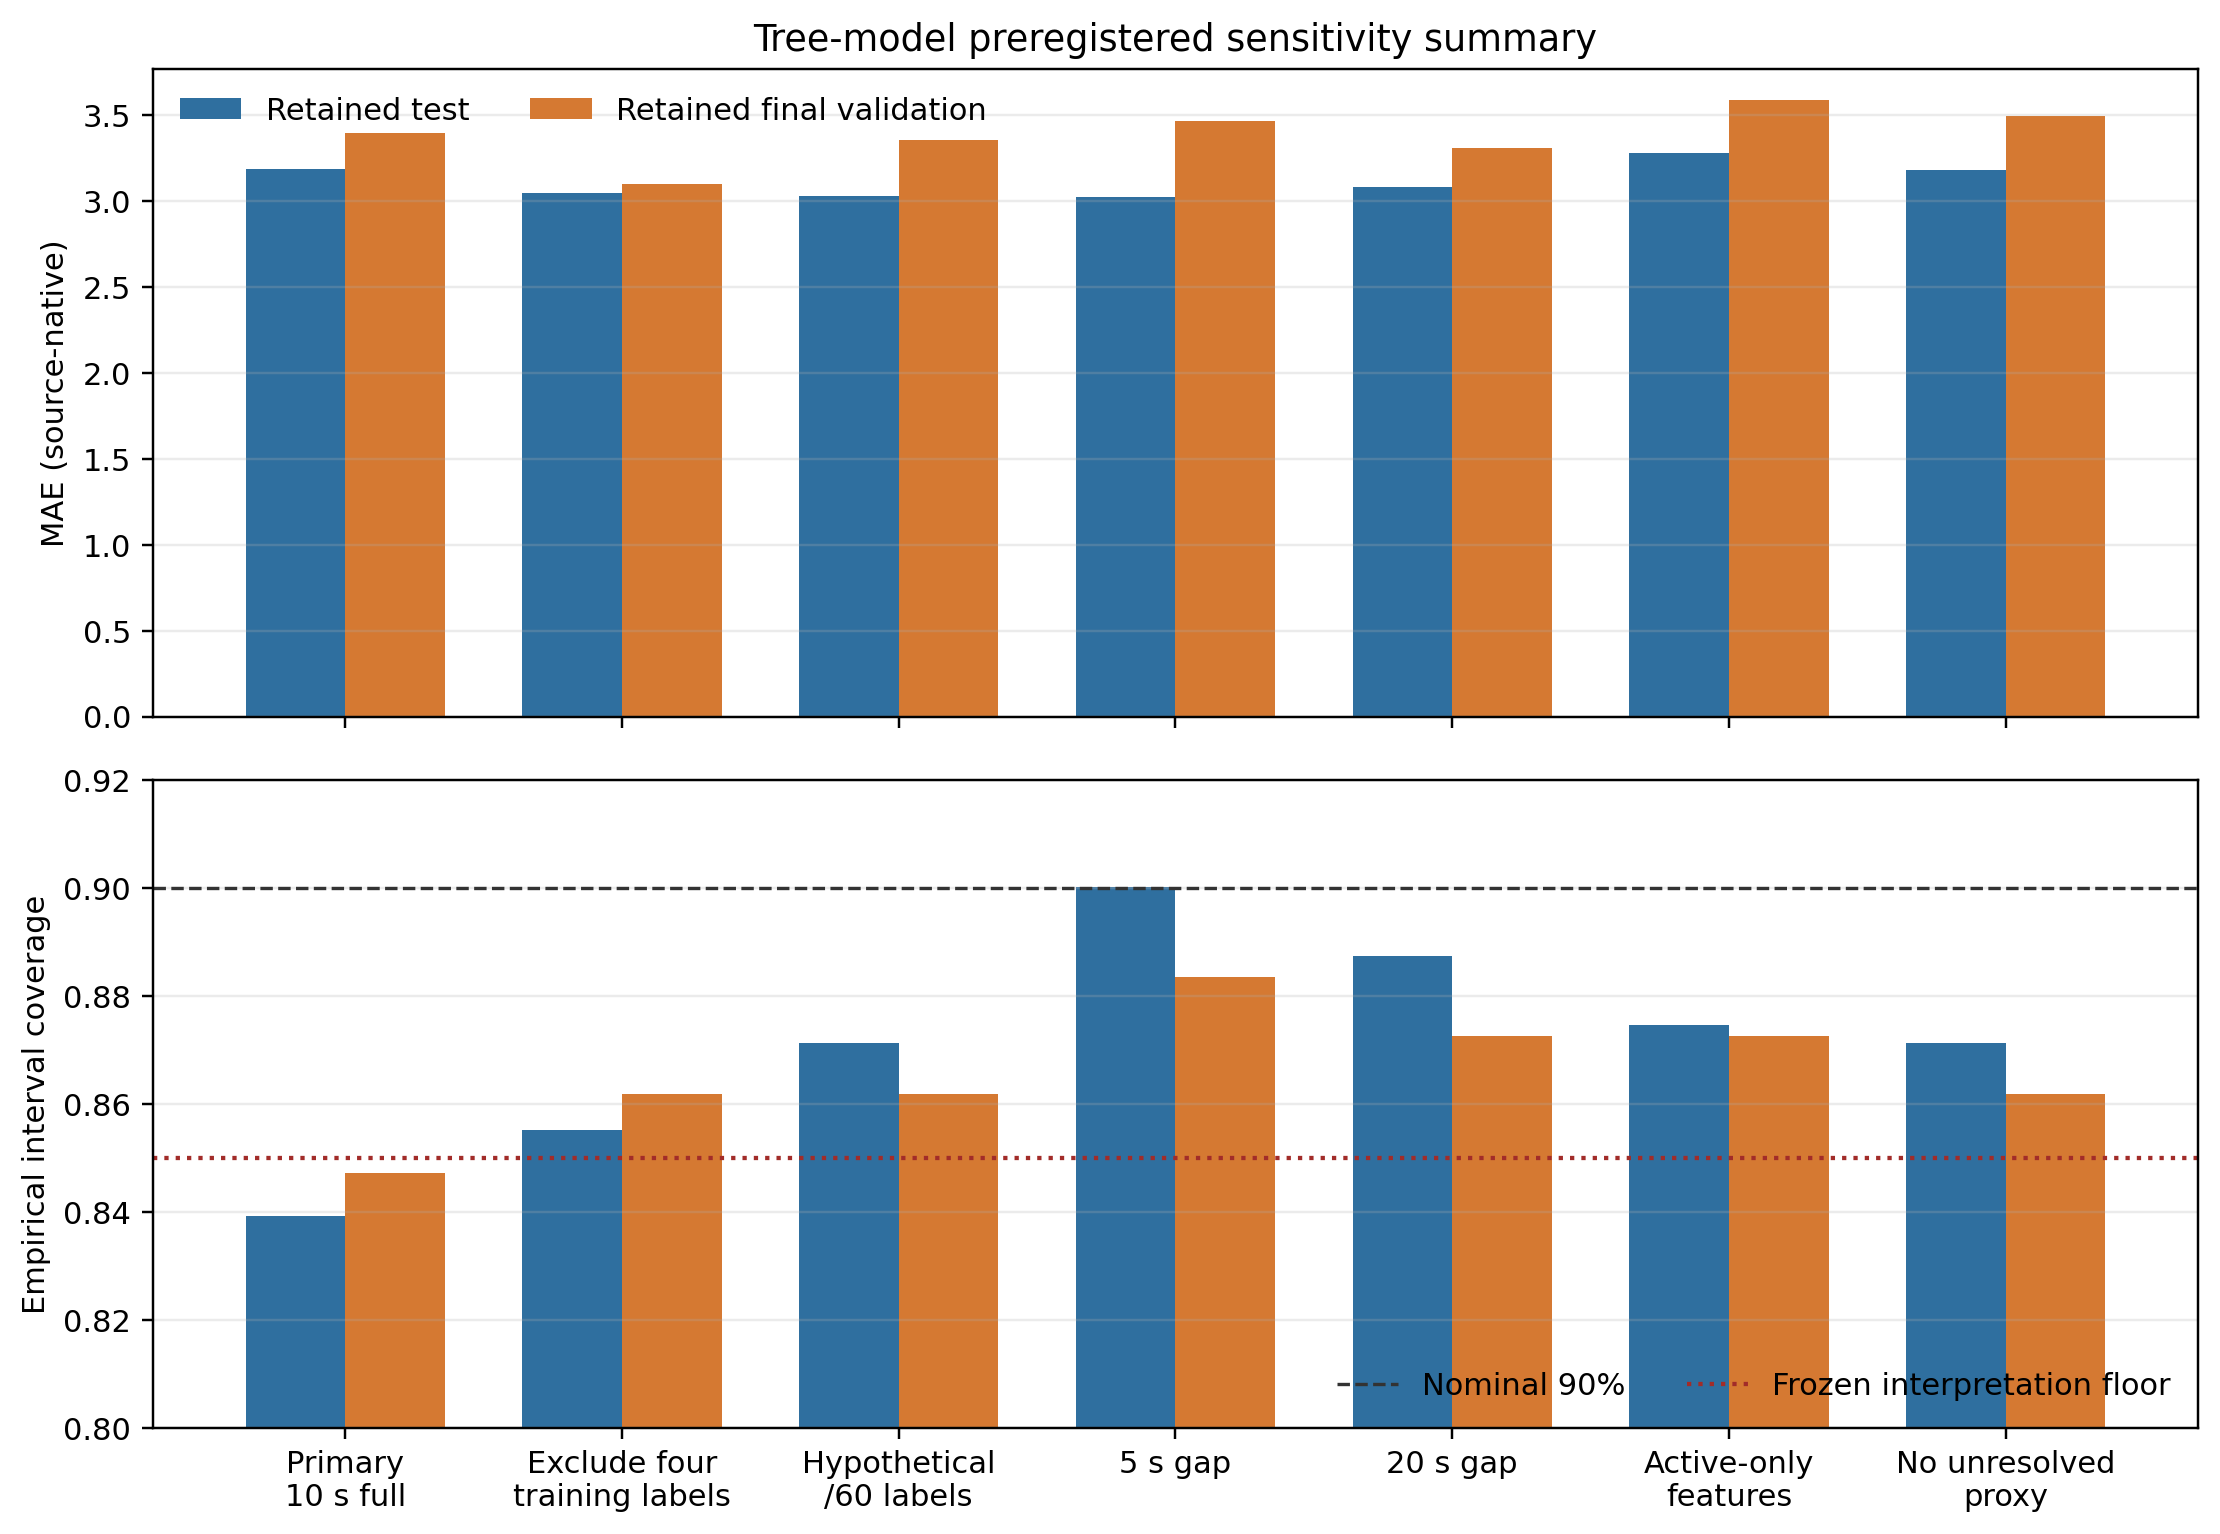
\includegraphics[width=0.91\textwidth]{wp09_tree_sensitivity.png}
\caption{Preregistered tree sensitivities. Point MAE is stable across declared
label, continuity, and feature-proxy variants, whereas empirical interval
coverage changes materially. The dashed line is nominal 90\% and the dotted
line is the frozen 85\% interpretation floor.}
\label{fig:wp09-sensitivity}
\end{figure*}

Consumable-feature removal worsens tree MAE but improves ridge MAE, so the
cross-model association gate fails and no causal degradation claim is made.
Chronological stress is also severe: tree MAE/RMSE become 18.50/239.84 with
$R^2=0.037$ and coverage 0.812. Median absolute error remains 3.19, but one
preregistered extreme late-block label (target 4326.154 versus prediction
152.927 and late-block median target 83.309) dominates the tail. No post-hoc
exclusion model was fitted. Machine generalization remains infeasible because
all records expose the same machine identifier.

\subsection{WP12: early-warning target and models}

Let $R_k$ be disturbed true simulated instantaneous average MRR and
$R_k^{\mathrm{ref}}$ the event-disabled paired reference at the same step. The
reference preserves initial state, schedule, declared topology, and static
plant parameters. The frozen point-violation indicator is
\begin{equation}
\begin{aligned}
v_k={}&\mathbb I[m_k=\textsc{polish}]
\mathbb I[R_k^{\mathrm{ref}}>10^{-12}\,\mathrm{m/s}]\\
&\times\mathbb I[R_k<0.95R_k^{\mathrm{ref}}
\;\lor\;R_k>1.05R_k^{\mathrm{ref}}].
\end{aligned}
\label{eq:warning-violation}
\end{equation}
An episode requires
$n_p=\lceil0.25\,\mathrm{s}/0.01\,\mathrm{s}\rceil=25$ consecutive
active-POLISH violating intervals. Its onset is the first interval of the
subsequently persistent departure. Other modes cannot create an event merely
because their MRR is zero.

At eligible 0.10 s decision time $t_d$, with $H=3.0$ s, the offline label is
\begin{equation}
y(t_d)=\mathbb I[t_d<t_e\leq t_d+H],
\label{eq:warning-target}
\end{equation}
where $t_e$ is the first accepted onset. Rows are censored instead of made
negative if the full horizon is absent, no 0.25 s contiguous active-POLISH
opportunity exists, or onset has already occurred.

Only observations satisfying $t_{\mathrm{arrival}}\leq t_d$ and
$k_{\mathrm{source}}\leq k_d$ enter the 65-feature vector. Eight observed
channels cover grid voltage, UPS output/battery, motor speed, pump flow, UPW
pressure/tool flow, and UPW temperature. Each contributes latest value and
age, 0.5 s mean/minimum/slope/missing fraction, and history minimum. UPS
output, pressure, and tool flow also use arrived-history deficit
\begin{equation}
D_j(t_d)=\int_0^{t_d}\max(0,0.95-z_j(t))\,dt.
\label{eq:warning-deficit}
\end{equation}
Known synthetic schedule indicators and static battery/load ratios are
permitted. MRR, latent pad/coupling state, event family or cause, and future
truth are prohibited. Imputation and scaling fit TRAIN only.

Whole runs are disjoint across TRAIN (2,988 eligible/84 positive rows),
probability CALIBRATION (1,404/84), independent
CONFORMAL\_CALIBRATION (1,404/84), and TEST (1,932/84). The 84 positive TEST
rows are 28 warning decisions around each of only three event-bearing runs.
The frozen comparison uses a training-prevalence constant, balanced logistic
regression, and balanced histogram gradient boosting. No TEST metric tunes a
model or selects one for sensitivity/robustness analysis.

With calibrated probability $\tilde p_i$, independent conformal rows use
\begin{equation}
s_i=\begin{cases}
1-\tilde p_i,&y_i=1,\\
\tilde p_i,&y_i=0,
\end{cases}
\label{eq:warning-conformal}
\end{equation}
and the prediction set is
\begin{equation}
\begin{aligned}
\Gamma(x)={}&\{0:\tilde p(x)\leq\hat q\}\\
&\cup\{1:1-\tilde p(x)\leq\hat q\}.
\end{aligned}
\label{eq:warning-set}
\end{equation}
where $\hat q$ is the finite-sample higher quantile at $\alpha=0.10$.
Temporal dependence and fixed severity grids make coverage an empirical
row-level simulator diagnostic, not a run-wise or real-world guarantee.

\begin{table*}[t]
\centering
\caption{Primary held-out WP12 warning results. One false-alarm episode over
193.2 eligible simulated seconds is 18.63 per eligible simulated hour; this is
not a real-fab alarm rate.}
\label{tab:wp12-primary}
\small
\begin{tabular}{lrrr}
\toprule
Metric & Prevalence & Logistic & Gradient boosted\\
\midrule
PR-AUC (prevalence 0.04348) & 0.04348 & 0.99040 & 0.91304\\
Precision & undefined & 0.97500 & 0.91304\\
Row recall & 0.00000 & 0.92857 & 1.00000\\
Specificity & 1.00000 & 0.99892 & 0.99567\\
Brier score & 0.04186 & 0.00321 & 0.00678\\
Event recall & 0/3 & 3/3 & 3/3\\
Median warning lead (s) & undefined & 2.71 & 2.71\\
False-alarm episodes & 0 & 1 & 1\\
Conformal coverage & 0.95652 & 0.92961 & 0.87733\\
Empty-set fraction & 0.00000 & 0.07039 & 0.12267\\
\bottomrule
\end{tabular}
\end{table*}

\begin{figure*}[t]
\centering
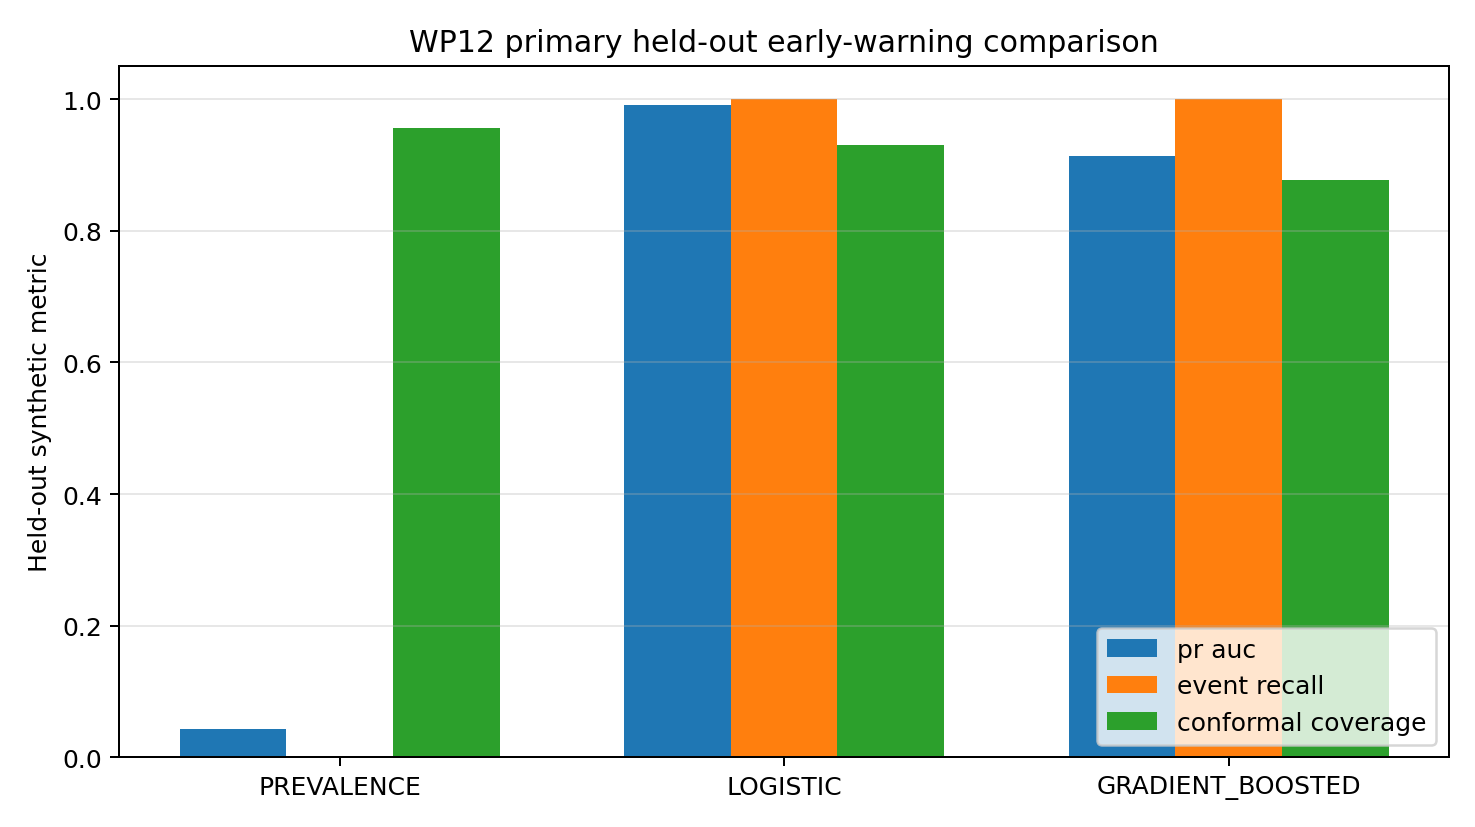
\includegraphics[width=0.47\textwidth]{wp12_model_comparison.png}\hfill
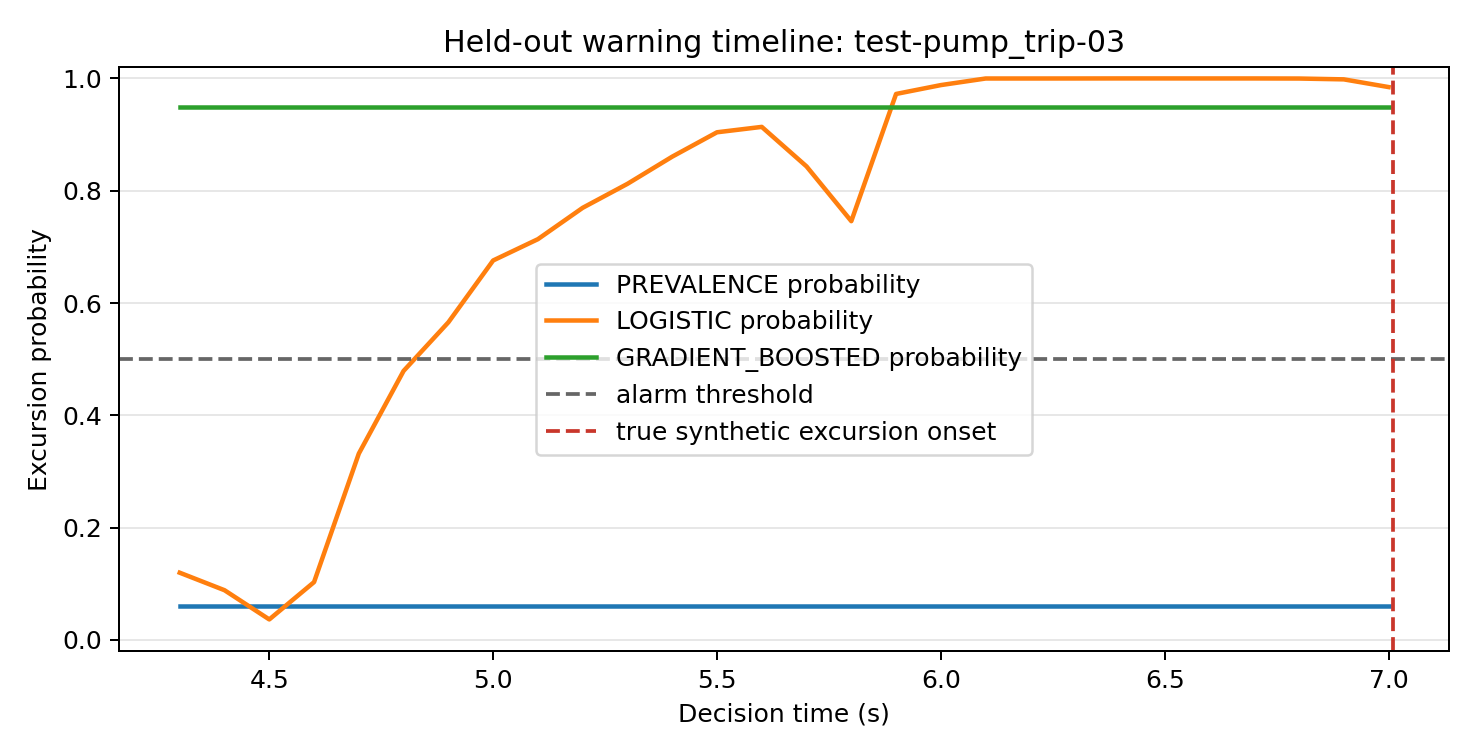
\includegraphics[width=0.47\textwidth]{wp12_warning_timeline.png}
\caption{Frozen WP12 synthetic results. Left: held-out discrimination,
event accounting, and empirical conformal summaries. Right: all three frozen
probability trajectories on one event-bearing held-out run. These are
open-loop simulator results, not a control comparison.}
\label{fig:wp12-results}
\end{figure*}

Both learned models pass the four frozen primary gates, but the gate has no
false-alarm acceptance threshold and event recall rests on three events. The
structural-null set has zero true events, yet logistic regression raises 30
false-alarm episodes (specificity 0.3371) and gradient boosting nine
(specificity 0.2860). Under high synthetic noise, logistic PR-AUC/precision/
specificity/coverage become 0.6002/0.1019/0.0657/0.0959; gradient boosting
gives 0.5283/0.5283/0.9053/0.7671. These failures show that upstream severity
can be learned without proving downstream CMP applicability. WP15/WP16 must
therefore gate topology, sensor validity, uncertainty, and model envelope.

\subsection{WP13: root-cause attribution}

\pending{}: candidate initiating classes are grid voltage sag, UPS transfer,
VFD derating, pump trip, valve restriction, tool-demand spike, thermal
excursion, pressure-sensor fault, flow-sensor fault, and unknown. Simulator
initiating labels are available only for offline scoring. The runtime method
will combine mechanistic residual checks, causal-chain rules, and cautious
feature attribution. Propagation states will not replace initiating causes,
compound events will preserve ordered multi-label truth, and uncertainty or
conflict will map to \textsc{unknown}. Results require a held-out confusion
matrix and class-conditional uncertainty; feature importance alone will not be
treated as causal identification.

\subsection{WP14--WP16: baselines, predictive supervision, and safety}

\pending{}: baselines will include no action, fixed threshold with hysteresis,
safe hold, and controlled resume. The first predictive supervisor will use
bounded action search or short-horizon model-predictive control, not
reinforcement learning. Candidate actions are no action, bounded VFD or valve
adjustment, bounded downforce/head/platen-speed reduction, advisory warning,
safe hold, and controlled resume.

The optimization objective must jointly penalize predicted active-polish MRR
deviation, cumulative-removal error, action effort and slew, hold duration,
recovery time, and throughput cost. Coefficients, horizon, terminal treatment,
and infeasibility behavior remain to be frozen. Cumulative removal and active
time from Eq.~\eqref{eq:cumulative-removal} prevent a hold-only policy from
gaming instantaneous-MRR error.

An independent safety filter will evaluate the controller proposal after the
controller acts. It will check action magnitude, slew rate, sensor validity,
prediction uncertainty, approved simulation envelope, and restart conditions.
Its auditable outcomes are \textsc{approved}, \textsc{clipped},
\textsc{rejected-out-of-envelope}, \textsc{rejected-sensor-invalid},
\textsc{rejected-high-uncertainty}, and \textsc{replaced-with-hold}. A claim
that final simulated actions remain within configured limits requires
exhaustive rejection-path and property tests with zero final-action violations.
It would be a software/simulation property, not equipment certification.

\subsection{WP17--WP18: integrated paired evaluation}

\pending{}: no action, threshold control, and predictive control will be run
on identical scenarios, initial states, parameter draws, seed maps, and sensor
corruptions. A manifest equality assertion will differ only in controller
identity and the trajectories subsequently caused by its actions. The final
comparison will include normal, mild and severe electrical disturbances, UPS
transfer, pump trip, valve restriction, demand spike, temperature event,
sensor bias/dropout, recoverable and hold-required disturbances, slow drift,
and compound unseen cases.

Metrics will include peak and integrated active-polish MRR deviation,
cumulative-removal error, pressure/flow violation duration, warning time,
false alarms, missed events, hold and recovery duration, action magnitude,
safety-filter rejections, attribution accuracy, prediction/controller latency,
and simulation throughput. Summaries will report mean, median, standard
deviation, 5th and 95th percentiles, and worst case. A controller-benefit claim
also requires preregistered paired success and non-inferiority criteria; no such
claim is made here.

\begin{table*}[t]
\centering
\caption{Manuscript evidence status at the WP09/WP12 freeze. ``Protocol'' means the
method is described but no performance result is asserted.}
\label{tab:status}
\small
\begin{tabular}{p{0.12\textwidth}p{0.19\textwidth}p{0.14\textwidth}p{0.43\textwidth}}
\toprule
Work package & Topic & Status & Current manuscript treatment\\
\midrule
WP03/R2 & PHM data pipeline & Verified contract & Provenance, semantics, native-unit and split policy\\
WP04--WP07/R3--R4 & Utility, sensing, timing & Synthetic checks complete & Equations, conservation, causal observation contract\\
WP08 & CMP physics & Synthetic checks complete & Reference, limiting, energy, timestep, replay results\\
WP10 & Utility--CMP coupling & Synthetic checks complete & Null/positive chain and sensitivity results\\
WP09 & Virtual metrology & Public-data result & Six-family comparison, grouped uncertainty, sensitivities and failed gates\\
WP12 & Early warning & Synthetic result & Frozen target, causal features,
disjoint calibration, primary and shift results\\
WP13 & Attribution & Protocol & Classes, unknown policy, evidence combination\\
WP14--WP16 & Control and safety filter & Protocol & Bounded actions, objectives, independent validation plan\\
WP17--WP18 & Integrated comparison & Protocol & Paired-run and robustness plan\\
\bottomrule
\end{tabular}
\end{table*}

\section{Discussion}

The most important modelling result is not the magnitude of the positive case
but the mechanism and its controls. A direct UPW-to-MRR multiplier would make
MRR respond even outside active polishing, hide whether utility water actually
connects to the tool process, and allow a gain to manufacture the desired
causal chain. In the present topology, electrical loss first depletes a
synthetic UPS, then changes drive, pump, and conserved UPW states. Only a
declared dressing branch changes CMP boundary availability; the pad activity
state stores that history; and MRR changes only during subsequent polishing.
The healthy-sag null case and exact zero-link equivalence are as important as
the positive chain because they constrain model freedom.

The 3.19\% decrease is a within-simulator paired difference, not an estimate of
what any real CMP tool would experience. Global sensitivity assigns substantial
conditional influence to link strength and reference pressure, while mismatch
cases span the no-connection result. This means topology and coupling
uncertainty must be propagated into later warning and controller studies. A
predictive policy that succeeds only when an assumed link is strong may fail
under no connection or a different plumbing path; later evaluation must retain
those structural nulls rather than optimize them away.

WP12 makes that warning concrete but also demonstrates the applicability
problem. Primary held-out separation is high and both learned models warn of
all three configured events 2.71 s in advance at the median. However, the
severe anchors repeat a narrow full-DRESS service-loss mechanism, so 84
positive decision rows do not constitute 84 independent events. Whole-run
bootstrap intervals resample only the same 24 configured TEST runs and cannot
create missing physical diversity.

More importantly, the no-connection diagnostic breaks the implication from
upstream severity to downstream MRR: the models alarm frequently while the
primary MRR target remains negative. High noise also produces poor
discrimination, false alarms, and empty conformal sets. A prediction score is
therefore neither root-cause proof nor permission to actuate. This negative
result directly constrains WP15/WP16: applicability and uncertainty failures
must reject the proposal or replace it with a safe hold, independently of
nominal TEST accuracy.

The explicit evidence-plane separation is equally consequential for virtual
metrology. Public PHM features are scaled and the target unit is not declared
by the original source. The simulator can still supply hypotheses and
dimensionless structures, but an SI Preston term cannot become a public-data
physics residual baseline merely by matching a number. Model comparison must
remain native-unit and leakage-safe until a defensible unit/calibration bridge
exists. Within that boundary, the tree supplies a strong offline point model,
but the physics proxy and hybrid results are cautionary: structural plausibility
does not guarantee predictive improvement when units and physical calibration
are absent. The hybrid's significantly worse error blocks the intended
physics-plus-residual claim rather than being hidden behind the tree result.

The public-data uncertainty and chronology findings also separate point
accuracy from reliability. The primary tree's narrow symmetric intervals
undercover both retained roles, and an extreme late-block target collapses
chronological RMSE despite a small median error. Label and continuity
sensitivities show that both coverage and tail behaviour depend on defensible
data semantics. A controller or safety filter therefore cannot treat the
WP09 interval as an approved operating bound, nor can it assume the random
whole-wafer split establishes future temporal performance.

Finally, the study treats supervisory safety as an independent software
contract, not as a property inferred from predictive accuracy. An accurate
warning model can still propose an infeasible action, act on an invalid sensor,
or resume too early. Keeping the safety filter separate enables explicit
rejection, clipping, hold fallback, and restart tests. Those results remain
future work.

\section{Limitations and threats to validity}

\begin{itemize}
  \item The PHM archive has verified local provenance, but its embedded dataset
  licence is not separately stated. Its target unit is source-undeclared and
  process scaling factors are hidden.
  \item Process-mode proxies are inferred from inputs, 306 official
  wafer/stage groups remain unresolved across splits, four extreme training
  labels require preregistered sensitivity analyses, and all records use one
  machine ID.
  \item The source partitions reuse wafer IDs across roles; only the
  precedence-retained roles support the primary independent-wafer comparison.
  The selected tree's nominal 90\% intervals cover only 83.9\%/84.7\%, and
  one known extreme label dominates the chronological stress RMSE.
  \item PHM data do not contain paired electrical/UPW utility histories and
  therefore cannot validate the proposed utility-to-CMP causal chain.
  \item UPS, VFD, motor, pump, UPW compliance, thermal, and sensor/network
  dynamics are reduced-order engineering approximations with synthetic
  capacities, coefficients, delays, and disturbances.
  \item The pump lacks manufacturer curves, efficiency maps, best-efficiency
  point, cavitation/NPSH, shaft loss at runout, and motor-load feedback. The
  hydraulic model omits distributed inertia and water hammer.
  \item The water-quality state is a dimensionless synthetic deviation, not
  measured chemistry or contamination. It has no CMP coupling.
  \item CMP uses spatially uniform pressure and reduced-order spindle, slurry,
  thermal, pad, wear, and dresser states. Numerical parameters are synthetic,
  not calibrated to a material/tool stack.
  \item The default temperature-to-MRR coefficient is zero. Thermal coupling
  is therefore a structural null for MRR in the default material profile.
  \item The reviewed literature supports pathway plausibility, not the target
  tool plumbing or numerical header thresholds. No-connection and zero-link
  cases remain scientifically necessary.
  \item Scenario labels and parameter distributions are synthetic definitions,
  not observed fab fault rates. Simulator truth supports internal scoring only.
  \item Primary WP12 TEST evidence has only three independent event-bearing
  runs. Positive endpoints require nearly full-DRESS synthetic service loss,
  and fixed severity grids are not samples from a fab distribution.
  \item Both learned warning models false-alarm severely under explicit
  no-connection and unseen-compound shifts. High synthetic noise damages
  discrimination, specificity, calibration, and empirical conformal coverage.
  \item Probability and conformal calibration use disjoint whole runs, but
  temporal dependence prevents a formal run-level guarantee. Empty prediction
  sets occur on 7.04\% of logistic and 12.27\% of gradient-boosted primary
  rows and require independent high-uncertainty handling.
  \item Known schedule, battery capacity, and load are simulator configuration;
  real availability is unverified. Reported WP12 timing is vectorized offline
  inference, not streaming controller latency.
  \item Public-data virtual metrology is an offline source-native result only.
  Attribution, controller, safety-filter, integrated-runtime, and controller-
  robustness results are unavailable at this evidence freeze.
  \item No measured spatial metrology, physical-defect label, wafer-yield
  outcome, equipment trial, or real actuator interface is present. The work
  does not support defect, yield, equipment-damage, or production-control
  conclusions.
  \item A 10 ms synthetic timestep and eventual measured software latency must
  not be represented as a microsecond or production real-time guarantee.
\end{itemize}

\section{Reproducibility and traceability}

The Python environment is the project-local conda environment
\texttt{devkki}. The WP08 reference trace contains 700 rows and has SHA-256
\texttt{902fa428\ldots 75626e}; its canonical runtime configuration hash is
\texttt{99d7876e\ldots e91670}. WP10 uses schema/interface versions
2.4.0/3.2.0 and runtime hash
\texttt{b2b07edb\ldots d7383f}. The frozen negative-control and positive-chain
trace hashes are listed with their results above. The global sensitivity JSON
records estimator method, seed, ranges, raw indices, and parameter provenance.
WP12 uses experiment revision \texttt{1.4-no-test-selection}; its configuration
hash is \texttt{b5373001\ldots df1e05}, eligible-dataset hash is
\texttt{fabe232a\ldots b43fa}, and deterministic TEST/robustness probability
payload hash is \texttt{5a4fb701\ldots 0ede}. The payload excludes measured
latency and set-valued conformal outputs by design.

WP09 was opened from clean Git checkpoint
\texttt{01c59a6172\ldots e4358805463c}. Its target-blind split payload hash is
\texttt{44c88516\ldots 0ba944}; validation JSON and prediction CSV hashes are
\texttt{52d25cf9\ldots bd10c} and
\texttt{ea3e9e81\ldots 79826}; and the deterministic validation payload hash is
\texttt{84d4823b\ldots 320db}. All six model artifacts reload under checksum
verification. The result records CPython, NumPy, pandas, Pydantic, PyYAML, and
scikit-learn versions.

All six communication figures are generated from frozen CSV/JSON evidence. A
machine-readable manifest records input and output SHA-256 values and states
that it contains interim WP08/WP10 synthetic evidence only. This manuscript's
two WP12 figures are generated by the frozen early-warning validation driver
and have hashes \texttt{76863b51\ldots 53b16f} and
\texttt{077177e0\ldots 2dcfcb}. Three WP09 figures are regenerated from the
frozen JSON/CSV only; their input/output hashes and public-data claim boundary
are recorded in a separate figure manifest. The evidence map links each quantitative
statement to the governing report and artifact. The article is rebuilt locally with
\texttt{conda run -n devkki make paper}; intermediate LaTeX files remain under
\texttt{paper/build}, and the reviewed PDF is written under
\texttt{reports/paper}.

Immediately before WP09 target access, 19 focused tests passed; the complete
repository suite passed 192/192 with warnings treated as errors. These counts
are historical evidence tied to the frozen revisions, not a claim that future
changes automatically preserve the result. Reproducible paired controller
manifests and the final claims audit remain pending.

\section{Conclusion}

This work has established a bounded synthetic foundation for studying
electrical and UPW disturbances in CMP. The utility plant conserves accepted
UPS energy and UPW mass, the CMP subsystem respects process modes and stores
consumable/thermal history, and a typed connection makes the assumed physical
path explicit. The healthy-UPS sag remains a null, while a separately declared
degraded-UPS dressing event yields a delayed 3.19\% lower later simulated MRR
through pad activity. Sensitivity results show that this magnitude depends
materially on synthetic connection assumptions.

The detection half of the central question now has a narrow synthetic answer:
two frozen models anticipate all three configured primary events with useful
lead time. The structural-null and noise failures show why that result cannot
be interpreted as topology-independent causality or permission to act.
Separately, a leakage-safe public-data tree predicts source-native average MRR
well on retained whole-wafer holdouts, but interval undercoverage, a failed
hybrid claim, and chronological tail fragility prevent stronger reliability or
physical-model conclusions. The mitigation and safety half remains open until
held-out attribution, bounded control, independent safety filtering, and
paired robust evaluation are complete. Supported conclusions remain limited
to the retained PHM roles and to the tested synthetic equations, declared
topology, and named WP12 ensemble.

\section*{Data, code, and manuscript status}

The PHM archive was supplied locally and is not redistributed by the paper.
The repository retains extraction checksums, preprocessing manifests,
deterministic traces, figure hashes, tests, and the living evidence map. This
is a journal-neutral draft; authorship, affiliations, funding, competing
interests, acknowledgements, a target journal class, and submission-specific
data/code availability language must be completed before submission.

\bibliographystyle{unsrt}
\bibliography{references}

\end{document}
